\documentclass[12pt, a4paper, twoside, openright, english]{book}

\usepackage[english]{babel}
\usepackage[utf8]{inputenc}
\usepackage[T1]{fontenc}
\usepackage[top=2.5cm,
	bottom=3cm,
	right=3.2cm,
	left=3.2cm
]{geometry}

\usepackage{subcaption}
\usepackage{hyperref}
\usepackage{enumitem}
\usepackage{tabularx}
\usepackage{afterpage}
\usepackage{longtable}
\usepackage{multirow}
\usepackage{amsfonts}
\usepackage{amssymb}
\usepackage{listings}
\usepackage{titlesec}
\usepackage{setspace}
\usepackage{fancyhdr}
\usepackage{fancyvrb}
\usepackage[fleqn]{amsmath}
\usepackage{pdfpages}
\usepackage{nccmath}
\usepackage{csquotes}
\usepackage{diagbox}
\usepackage{ifthen}
\usepackage{algorithm}
\usepackage{algpseudocode}
\usepackage[super]{nth}

\usepackage[titles]{tocloft} % TOC header same as chapter title
%\usepackage{showframe}
\usepackage{titlesec}
\titlespacing*{\chapter}{0pt}{0pt}{40pt}

\usepackage{colortbl}
\usepackage{tabulary}
\usepackage{adjustbox}

\usepackage{lmodern}
\usepackage{fourier-orns}
\newlength\longest


\usepackage{nomencl}
\usepackage{makeidx}
\usepackage{expl3}
\usepackage{etoolbox}
%\preto\tabular{\shorthandoff{-}}

\usepackage[style=iso-numeric, backend=biber, url=false]{biblatex}
\renewcommand*{\bibfont}{\normalfont\small}
\addbibresource{literature.bib}

% Abbreviations
% \makenomenclature
% \renewcommand{\nomname}{List of Terminology and Abbreviations}

% Formulas
\newcommand{\listequationsname}{List of Equations}
\newlistof{myequations}{equ}{\listequationsname}
\newcommand{\myequations}[1]{
\addcontentsline{equ}{myequations}{\protect\numberline{\theequation}\quad #1}}

% Algorithms
\makeatletter
\renewcommand*{\ALG@name}{Algorithms}
%\renewcommand{\listalgorithmname}{Zoznam algoritmov}
\algrenewcommand\algorithmicrequire{\textbf{Input:}}
\algrenewcommand\algorithmicensure{\textbf{Output:}}
\makeatother

% Empty even pages at the end of chapter
\makeatletter
\renewcommand*{\cleardoublepage}{\clearpage\if@twoside \ifodd\c@page\else
\hbox{}%
\thispagestyle{empty}%
\newpage%
\if@twocolumn\hbox{}\newpage\fi\fi\fi}
\makeatother

% roman numerals
\makeatletter
\newcommand*{\rom}[1]{\expandafter\@slowromancap\romannumeral #1@}
\makeatother


% Číslo kapitoly na rovnakom riadku ako názov
\titleformat{\chapter}{\normalfont\huge\bf}{\thechapter}{1em}{}

\raggedbottom
\newcommand{\emptypage}{\newpage\thispagestyle{empty}\mbox{}\newpage}
\newcommand{\signaturespace}[2]{
  \begingroup
  \renewcommand{\arraystretch}{0}
  \begin{tabular}[t]{cc}
  \hspace*{0pt}
  \cleaders\hbox{\kern.6pt.\kern.6pt}\hskip#1\relax
  \hspace*{0pt}
  \\[0.5cm]
  #2
  \end{tabular}
  \endgroup
}

\pagestyle{fancy}
\fancyhf{}  % clear all header and footers
\fancyhead[LE]{\leftmark}
\fancyhead[RO]{\rightmark}
\fancyfoot[LE, RO]{\thepage}

\fancypagestyle{plain}{
  \fancyhf{}
  \renewcommand{\headrulewidth}{0pt}
  \fancyhf[lef,rof]{\thepage}
}

\setlength{\headheight}{16pt}

\renewcommand{\ttdefault}{pcr}
\lstdefinestyle{cstyle}{
    language=C,
	basicstyle=\linespread{1.1}\ttfamily\footnotesize,
    numbers=left,
    numberstyle=\tiny,
    frame=single,
    tabsize=4,
    captionpos=b,
    breaklines=true,
    texcl=true,
	numbersep=8pt,
	framexleftmargin=15pt,
	xleftmargin=5ex,
     xrightmargin=3.4pt,
	 morekeywords = {uint8_t,uint16_t,int16_t,uint32_t,int32_t,bool}
}
\lstdefinestyle{docs}{
    language=C,
	basicstyle=\linespread{1.1}\ttfamily\small\bfseries,
    tabsize=4,
    breaklines=true,
    belowskip=0pt
}
\renewcommand{\lstlistingname}{Source code}

\setstretch{1.5}
\newcommand{\University}[0] {Slovenská technická univerzita v Bratislave}
\newcommand{\UniversityEN}[0] {Slovak University of Technology in Bratislava}
\newcommand{\Faculty}[0] {Fakulta informatiky a informačných technológií}
\newcommand{\FacultyEN}[0] {Faculty of Informatics and Information Technologies}

\newcommand{\ThesisTitle}[0] {Diplomová práca}
\newcommand{\ThesisTitleEN}[0] {Master's thesis}

\newcommand{\Thesis}[0] {Diplomová práca}
\newcommand{\ThesisEN}[0] {Master's Thesis}
\newcommand{\Title}[0] {Vibrodiagnostika strojov s~priemyselným internetom vecí}
\newcommand{\TitleEN}[0] {Machinery Vibrodiagnostics with~the~Industrial~Internet~of~Things}

\newcommand{\Author}[0] {Bc. Miroslav Hájek}
\newcommand{\Supervisor}[0] {Ing. Marcel Baláž, PhD.}
\newcommand{\DepartmentalAdvisor}[0] {Ing. Jakub Findura}
\newcommand{\Consultant}[0] {Ing. Lukáš Doubravský}

\newcommand{\AuthorEN}[0] {Miroslav Hájek}
\newcommand{\SupervisorEN}[0] {Dr. Marcel Baláž}
\newcommand{\DepartmentalAdvisorEN}[0] {Jakub Findura}
\newcommand{\ConsultantEN}[0] {Lukáš Doubravský}

\newcommand{\RegNo}[0] {FIIT-xxxx-xxxxxx}
\newcommand{\Date}[0] {Máj 2024}
\newcommand{\DateEN}[0] {May 2024}
\newcommand{\SignDateEN}[0] {4 May 2024}
\newcommand{\StudyProgramme}[0] {Inteligentné softvérové systémy}
\newcommand{\StudyProgrammeEN}[0] {Intelligent Software Systems}
\newcommand{\StudyField}[0] {Informatika}
\newcommand{\StudyFieldEN}[0] {Computer Science}
\newcommand{\Institute}[0] {Institute of Computer Engineering and Applied Informatics}
\newcommand{\SignPlace}[0] {Bratislava, }

% Todo list
\newlist{todolist}{itemize}{2}
\setlist[todolist]{label=$\square$}


\begin{document}
\nomenclature{\textbf{Pojem}}{Vysvetlenie}
% Cover -------------------------------------------------------------
\thispagestyle{empty}
{\centering
	{\Large \UniversityEN}\par
	{\Large \FacultyEN}\par
	\vspace{\medskipamount}
	\RegNo
	\vfill
	\textbf{\Large \Author}\par
	\vspace{1.5\bigskipamount}
	\textbf{\LARGE \TitleEN}\par
	\vspace{1.5\bigskipamount}
	{\Large \ThesisEN}\par
	\vfill
}
\begin{flushleft}

{\large Thesis Supervisor: \Supervisor \\
\DateEN}
\end{flushleft}
\emptypage

%  Main part ------------------------------------------------------
\newgeometry{top=2.5cm, bottom=3cm, right=2.5cm, left=3.5cm}

% Title page
\pagenumbering{roman}
\thispagestyle{empty}
{\centering
	{\Large \UniversityEN}\par
	{\Large \FacultyEN}\par
	\vspace{\medskipamount}
	Reg. No. \RegNo
	\vfill
	\textbf{\Large \Author}\par
	\vspace{1.5\bigskipamount}
	\textbf{\LARGE \TitleEN}\par
	\vspace{1.5\bigskipamount}
	{\Large \ThesisEN}\par
	\vfill
}
\begin{flushleft}
\begin{longtable}[l]{ll}
Study programme: & \StudyProgrammeEN \\
Study field: & \StudyFieldEN \\
Training workplace: & \Institute\\
Thesis supervisor: & \Supervisor \\
Departmental advisor: & \DepartmentalAdvisor \\
Consultant: & \Consultant \\
\end{longtable}
\indent\DateEN
\end{flushleft}
\emptypage

% Thesis assignment
\thispagestyle{empty}

\includepdf[pages=-, scale=1]{chapters/assignment}
\emptypage

% Declaration of Honour
 % Declation of Honour
\thispagestyle{empty}
\vspace*{\fill}
\section*{Declation of Honour}

I hereby declare on my honour that I wrote this thesis independently under supervision of Dr. Marcel Baláž, after consultations and with use of cited literature.

\vspace{3\medskipamount}\noindent
\SignPlace \SignDateEN \hspace*{\fill} \signaturespace{5cm}{\Author} 

\emptypage

% Acknowledgments
% Poďakovanie
\thispagestyle{empty}
\vspace*{\fill}
\section*{Acknowledgement}

\vspace{3cm}
\emptypage

% Annotations
\thispagestyle{empty}
\section*{Annotation}
\UniversityEN \\
\uppercase{\FacultyEN}
\vspace{-8pt}
{\setlength{\mathindent}{0cm}
\begin{align*}
&\text{Degree course:} && \text{\StudyProgrammeEN} \\
&\text{Author:} && \text{\Author} \\
&\text{\ThesisEN:} && \text{\TitleEN} \\
&\text{Supervisor:} && \text{\SupervisorEN} \\
&\text{\DateEN}
\end{align*}}

\emptypage 

\thispagestyle{empty}
\section*{Anotácia}
\University \\
\uppercase{\Faculty}
\vspace{-8pt}
{\setlength{\mathindent}{0cm}
\begin{align*}
&\text{Študijný program:} && \text{\StudyProgramme} \\
&\text{Autor:} && \text{\Author} \\
&\text{\Thesis:} && \text{\Title} \\
&\text{Vedúci diplomovej práce:} && \text{\Supervisor} \\
&\text{\Date}
\end{align*}}

\emptypage

% Contents
\pagestyle{empty}
\tableofcontents{}
\listoffigures
\listoftables
\listofmyequations

% TODO: generate https://tex.stackexchange.com/questions/242129/can-not-print-nomenclature-in-texmaker
{\let\clearpage\relax \printnomenclature}
\emptypage

\pagestyle{fancy}
% Chapters
\pagenumbering{arabic}

\chapter{Introduction}
Manufacturing is experiencing a shift in the traditional practices of asset operational status evaluation and utilization. The rise of Industry 4.0 means greater automation and robotization of the production halls to achieve optimal usage of available resources. The secondary aspect in the enterprises' endeavor, however not less important, is to keep track of the equipment wear and tear. The corrective action be it repair or replacement should be taken on time in response to the key indicators. 

The goal is to preserve required safety and production efficiency when extending the useful life of machine moving parts. In the factories and logistics where this sort of equipment is vital, there is a rising interest in the ability to monitor in real-time the health of the machines and to proactively diagnose the fault to repair it without adding unnecessary costs. 

Vibrations are the most nonintrusive way with which such faults can be sensed. The experts use it to distinguish faulty states and to identify the malfunction's root cause. In critical circumstances such as in the case of the large turbines in the power plants, the precautions leading to regular machinery check-ups are already in place. To reach wider acceptance and spread, the monitoring solution has to be sufficiently independent, reliable, and as self-sufficient as the model design allows it to be.

The main issue to consider in large-scale machinery monitoring using vibrations are lots of uninformative streams of samples not directly useful for the production line operator. The dashboard must aggregate these flows into trend variables with severity levels categorized based on industrial standards. The majority of signals are viewed once at the maximum therefore to store or even transmit them from the edge device in its entirety would be wasteful. The complex overview of the mechanical equipment status is attainable only when agent devices and sensors are cheap enough with a long lifespan on battery power and preferably remain physically small to reduce the additional clutter.

Attempted machine and deep learning approaches have the crucial impediment that the construction of every single machine is unique to some extent because of tolerances and variable load. The model must be trained specifically for the target environment to achieve the ideal performance. In addition, the failures are relatively rare events occurring usually in the span of multiple months. In these circumstances, it is hard to obtain a large enough sample of fault events quickly. Novelty detection is a technique that can be applied in this case.

The thesis is organized in the following manner. In the first chapter of analysis in section 1 we explore the mechanical maintenance approaches and industry standards on common fault identification. Then section 2 is all about measuring vibrations and transforming them into features meaningful in automatic fault pattern recognition. In section 3 we delve into modes of diagnosis based on reduced relevant indicators. Section 4 deals with evaluation datasets used to determine computational requirements
on IIoT infrastructure. Chapter 2 defines data format and proposes processing steps to diagnose the imminent failure and different fault types. The approach taken is evaluated and validated in Chapter 6. 
  

\chapter{Problem analysis} \label{chapter:problem-analysis}
In the problem analysis chapter we explore the feature engineering methods and machine learning algorithms for fault diagnostics. The basis we build upon is the domain knowledge of mechanical engineers in vibration signal measurement and its evaluation.

\section{Condition monitoring} \label{section:condition-monitoring}
All rotating machinery eventually fails because of the long-term strain on the individual parts, inadequate workmanship, installation, or operational procedures. In the end, these factors cause the equipment not to fulfill its intended functionality. Many instrumentation methods are practiced to reveal evolving faults: vibration and acoustic noise monitoring, electric supply line measurements, thermography, oil and particle analysis, ultrasonic testing, etc. Vibration signals are the preferred tool for rotating machinery monitoring \cite{mohanty_machinery_2015}.

The defect needs to be repaired or replaced, preferably without significant production downtime, further damage to the other attached elements, or any endangerment of the responsible personnel. The maintenance strategies are chosen according to the machine's importance as a result of its failure effect evaluation on the system. The guide to set appropriate maintenance procedures as outlined in the IEC~60706-2 standard, and involves reliability-centered maintenance analysis~\cite{el-thalji_predictive_2019}.

\subsection{Maintenance strategies}
There are three different approaches to maintenance across the industry: \textbf{reactive, preventive, and predictive}~\cite{scheffer_practical_2004}. In general, the more sophisticated methods are beneficial in a high-stakes environment. The unexpected machine shutdown can have a negative economic impact on the enterprise, resulting in decreased product quality and demands for spare parts to be ready in the supply inventory at all times. In certain situations, it suffices to utilize a simpler maintenance program, but the predictive maintenance gains attraction in the Industry 4.0 to optimize usage of assets~\cite{cinar_machine_2020}.

\textbf{Reactive maintenance} allows machinery to run until a complete failure. This is the most inappropriate way to maintain the production line, but it is straightforward enough. It requires a large stock of replacement parts on-site and breakage inflicts a ``crisis management mode'' upon the plant \cite{scheffer_practical_2004}. On-demand repairs are justified when short downtime is acceptable, full and swift replacement of a broken machine with a backup is possible, or there is a negligible threat to the surrounding environment on failure~\cite{ziaran_technicka_2013}.

\textbf{Preventive maintenance} is performed before any issue is detected. Maintenance occurs at regular intervals derived from a predetermined period in the calendar or expected machine running time (MTTF - Mean Time To Failure). The schedule is crucial but can result in components being replaced in good condition creating waste. The parts can occasionally stay in operation too long, and the machine breaks as a result. Conservative planning is usually the norm to keep the machine always in a perfect state, and therefore more frequent interventions are required~\cite{mohanty_machinery_2015}.

\textbf{Predictive maintenance} known as condition-based maintenance (CbM), improves the predictability of reactive maintenance and eliminates the waste in overall resource utilization of cautious prevention. The machine downtime is scheduled after the detection of unhealthy trends in fault monitoring with sensors and the identification of troublesome components.

A measurable decrease in effectivity allows us to order necessary parts in advance and organize repairs of several machines at a convenient time. The misdetection leads to increased costs compared to previous methods and raises the expectation that faults are distinguishable among themselves~\cite{davies_handbook_2012}.

\begin{figure}[ht]
	\centering
	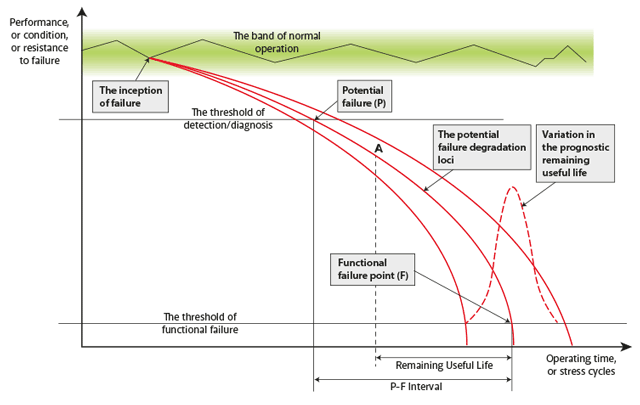
\includegraphics[width=\textwidth]{assets/P-F-Curve.png}
	\caption{P-F curve represents the evolution of the asset's health~\cite{jennions_integrated_2011}}
	\label{fig:p-f-curve}
\end{figure}

The \emph{P-F curve} is a widespread representation of equipment degradation over time based on historical records (Fig.~\ref{fig:p-f-curve}). Corrective action should be taken between the event of potential failure (P), when the fault detection is activated, and functional failure point (F) in the P-F interval~\cite{bousdekis_enterprise_2021}.  These division points are not exactly set but have statistical distribution to them.

The \emph{Remaining Useful Life} (RUL) of the specific running machine in the given instance can be merely estimated analytically, with the survival probabilities of the individual components, based on the model of the ``run-to-failure'' histories, and usage parameters~\cite{okoh_overview_2014}. Predictive condition monitoring aims to extend lifespan to the maximum by predicting expected RUL.

\begin{figure}[ht]
	\centering
	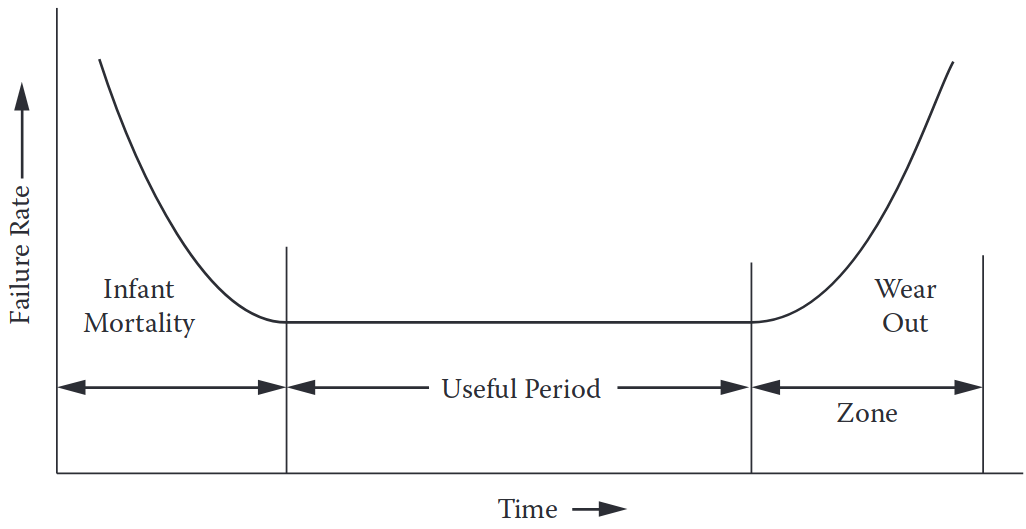
\includegraphics[width=0.6\textwidth]{assets/bath-tub-curve.png}
	\caption{Bathtub curve~\cite{mohanty_machinery_2015}}
	\label{fig:bathtub-curve}
\end{figure}

A high failure rate is present not only at the worn-out stage when the parts are fatigued or corroded but also in the early stages soon after assembly. Manufacturing or material defects, inadequate installation, or improper start-up procedures, are all suspected causes. During the stable middle phase, malfunction can occur after the machine's excessive overload. The time plot to failure rate is known as the bathtub curve~(Fig.~\ref{fig:bathtub-curve}).

\subsection{Vibration fault types}
Mechanical problems during machinery operation bring about vibrations in many instances. Therefore vibroacoustic diagnostics is considered as one of the most important methods in early component fault identification~\cite{ziaran_technicka_2013}.

The cause of vibration comes out of the changing force in its magnitude or direction. The most emerging defects can be encompassed by explaining the deficiencies of the mechanical structure. These defects are broadly categorized as \textbf{unbalance, misalignment, looseness, eccentricity, deformation, crack, and influence of the external force} (friction)~\cite{davies_handbook_2012}. It is important to stress that our concern is not the underlying deformities in mechanical parts, but the correct fault classification based on the signal waveform.

\begin{figure}[ht]
	\centering
	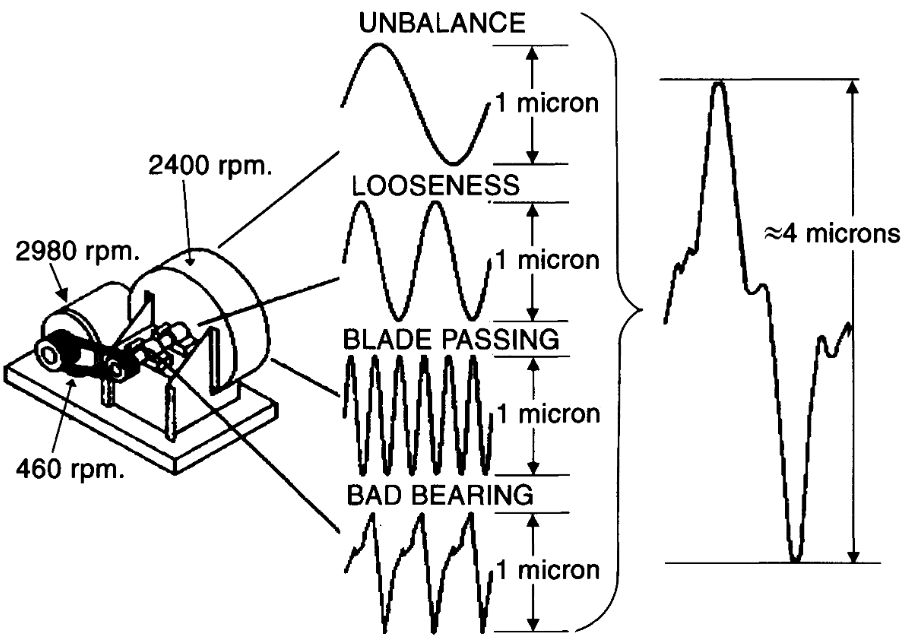
\includegraphics[width=0.6\textwidth]{assets/complex-vibrations.png}
	\caption{Complex machinery vibrations~\cite{davies_handbook_2012}}
	\label{fig:machinery-vibrations}
\end{figure}

Rotating machine disorders exhibit frequency signatures at various ranges in the frequency spectrum with supplementary symptoms carried in phase signal. Most of the occurring faults can be tied to the main rotational speed of the component under investigation (Fig.~\ref{fig:machinery-vibrations})~\cite{davies_handbook_2012}. Imbalance, misalignment, and looseness normally appear at frequencies up to 300 Hz. These low-frequency faults are associated with the movement of the shaft and primarily coincide with revolution speed and its harmonics. Bearing and gearbox defects in the late stages of development, show up in the range between 300 Hz and 1 kHz. Higher frequencies, measured traditionally to a limit of 10 kHz, help notice the faults in bearings even sooner~\cite{torres_automatic_2022}.

One of the methods vibration experts utilize in the identification of the damaged part from the frequency spectrum is \textbf{order analysis}. The excessive peaks at harmonic frequencies are of interest. Harmonics are integer multiples of fundamental frequency (1x rpm)~(Tab.~\ref{tab:vibration-causes}):

\begin{table}[h]
\renewcommand{\arraystretch}{1.2}
\begin{adjustbox}{width=\columnwidth,center}
\begin{tabular}{|ll|l|l|}
\hline
\multicolumn{2}{|l|}{\textbf{Frequency content}}                            & \textbf{Likely reason}                                                                                                     & \textbf{Other causes}                                                                                                                          \\ \hline
\multicolumn{1}{|l|}{\multirow{4}{*}{Synchronous}} & 1 x rpm                & Imbalance                                                                                                                & \begin{tabular}[c]{@{}l@{}}Eccentric journals\\ Bent shaft / Misalignment\\    (high axial vibration)\\ Bad belt (if rpm of belt)\end{tabular} \\ \cline{2-4}
\multicolumn{1}{|l|}{}                             & 2 x rpm                & Looseness                                                                                                                & \begin{tabular}[c]{@{}l@{}}Misalignment \\    (high axial vibration)\\ Cracked rotor\\ Bad belt (if rpm of belt)\end{tabular}                  \\ \cline{2-4}
\multicolumn{1}{|l|}{}                             & 3 x rpm                & Misalignment                                                                                                             & and axial looseness                                                                                                                             \\ \cline{2-4}
\multicolumn{1}{|l|}{}                             & Many x rpm             & \begin{tabular}[c]{@{}l@{}}Bad gears\\ Severe looseness\end{tabular}                                                     & \begin{tabular}[c]{@{}l@{}}Gear teeth x rpm\\ Fan blade count x rpm\end{tabular}                                                               \\ \hline
\multicolumn{1}{|l|}{Sub-synchronous}                 & \textless 1 x rpm      & Oil whirl                                                                                                                & \begin{tabular}[c]{@{}l@{}}Bad drive belt\\ Background\\ Resonance\end{tabular}                                                                \\ \hline
\multicolumn{1}{|l|}{Non-synchronous}              & \multicolumn{1}{c|}{-} & \begin{tabular}[c]{@{}l@{}}Electrical problems (x 50 Hz)\\ Reciprocating forces\\ Aerodynamic forces \\ Bad antifriction bearings\end{tabular} & Rubbing \\ \hline
\end{tabular}
\end{adjustbox}
\caption{Expert observed likely vibration causes (based on~\cite{davies_handbook_2012,ziaran_technicka_2013,noauthor_iso_2002})}
\label{tab:vibration-causes}
\end{table}

Because of inherent tolerances in machine manufacturing and assembly, the rotational frequency always manifests itself, even in baseline signature~\cite{davies_handbook_2012, noauthor_iso_2002}. In the most likely scenario, some faults appear as compared to rotational frequency solely in \textbf{synchronous, subsynchronous, or non-synchronous components}. The defects can occur in a predictable combination of the ones mentioned. Other common patterns experts look for are modulation sidebands typical for bearings and gears extractable with cepstrum analysis~\cite{ziaran_technicka_2013}. Procedures relying on elimination narrow down unrelated causes effectively.

\subsection{Technical standards}
Vibration-based condition monitoring practices adopted in the factory's predictive maintenance management must comply with normative guidelines formalized in ISO international standards. Standards are concerned with each step in the process that originates with transducer placements and data acquisition. They prescribe conventions for setting fault severity levels and provide empirically observed vibration characteristics of common defects. Relevant standards for IoT diagnostics systems are \emph{ISO 20816} (updated from ISO 10816) and \emph{ISO 13373}.
\bigbreak

\textbf{ISO 20816-1:2016} establishes the approaches of vibration measurement and evaluation on non-rotating housing of machinery parts~\cite{noauthor_iso_2016}. The measurement units are agreed upon for kinematic quantities of vibrations. Acceleration is measured in meters per second squared ($m/s^2$), velocity in millimeters per second ($mm/s$), and displacement in micrometers ($\mu m$). It is customary to evaluate broad-band vibration velocity in terms of root mean square value (rms), as it is related to signal energy. No simple direct relationship is expressible among these physical quantities, except in stationary signals.

The vibration severity is the maximum of magnitudes measured in two radial directions (horizontal, and vertical) or supplemented with a third direction along the shaft in the axial axis. Multiple measurement locations, i.e. on different bearings or couplings, should be assessed independently.

Criteria introduced to judge vibration severity are absolute vibration magnitude, change in the magnitude vector, and rate of change. In terms of maximal magnitudes, the machines of varied sizes are split into four severity zones defined in the chart ~(Tab.~\ref{tab:iso20816-vibration-severity}). The values in this table serve as guidelines towards realistic requirements between machine manufacturers and their customers.

\begin{table}[h]
\centering
\renewcommand{\arraystretch}{1.2}
\begin{adjustbox}{width=\columnwidth,center}
\begin{tabular}{|c|c|c|c|c|}
\hline
\textbf{\begin{tabular}[c]{@{}c@{}}Vibration velocity\\ RMS {[}mm/s{]}\end{tabular}} & \textbf{\begin{tabular}[c]{@{}c@{}}Class I\\ Small machines\end{tabular}} & \textbf{\begin{tabular}[c]{@{}c@{}}Class II\\ Medium machines\end{tabular}} & \textbf{\begin{tabular}[c]{@{}c@{}}Class III\\ Large machines\\ Rigid supports\end{tabular}} & \textbf{\begin{tabular}[c]{@{}c@{}}Class IV\\ Large machines\\ Flexible support\end{tabular}} \\ \hline
0.28                                                                                 & \cellcolor[HTML]{9AFF99}                                                  & \cellcolor[HTML]{9AFF99}                                                    & \cellcolor[HTML]{9AFF99}                                                                     & \cellcolor[HTML]{9AFF99}                                                                      \\ \cline{1-1}
0.45                                                                                 & \cellcolor[HTML]{9AFF99}                                                  & \cellcolor[HTML]{9AFF99}                                                    & \cellcolor[HTML]{9AFF99}                                                                     & \cellcolor[HTML]{9AFF99}                                                                      \\ \cline{1-1}
0.71                                                                                 & \multirow{-3}{*}{\cellcolor[HTML]{9AFF99}\textbf{Good (A)}}               & \cellcolor[HTML]{9AFF99}                                                    & \cellcolor[HTML]{9AFF99}                                                                     & \cellcolor[HTML]{9AFF99}                                                                      \\ \cline{1-2}
1.12                                                                                 & \cellcolor[HTML]{FFFC9E}                                                  & \multirow{-4}{*}{\cellcolor[HTML]{9AFF99}\textbf{Good (A)}}                 & \cellcolor[HTML]{9AFF99}                                                                     & \cellcolor[HTML]{9AFF99}                                                                      \\ \cline{1-1} \cline{3-3}
1.8                                                                                  & \multirow{-2}{*}{\cellcolor[HTML]{FFFC9E}\textbf{Satisfactory (B)}}       & \cellcolor[HTML]{FFFC9E}                                                    & \multirow{-5}{*}{\cellcolor[HTML]{9AFF99}\textbf{Good (A)}}                                  & \cellcolor[HTML]{9AFF99}                                                                      \\ \cline{1-2} \cline{4-4}
2.8                                                                                  & \cellcolor[HTML]{F8A102}                                                  & \multirow{-2}{*}{\cellcolor[HTML]{FFFC9E}\textbf{Satisfactory (B)}}         & \cellcolor[HTML]{FFFC9E}                                                                     & \multirow{-6}{*}{\cellcolor[HTML]{9AFF99}\textbf{Good (A)}}                                   \\ \cline{1-1} \cline{3-3} \cline{5-5}
4.5                                                                                  & \multirow{-2}{*}{\cellcolor[HTML]{F8A102}\textbf{Unsatisfactory (C)}}     & \cellcolor[HTML]{F8A102}                                                    & \multirow{-2}{*}{\cellcolor[HTML]{FFFC9E}\textbf{Satisfactory (B)}}                          & \cellcolor[HTML]{FFFC9E}                                                                      \\ \cline{1-2} \cline{4-4}
7.1                                                                                  & \cellcolor[HTML]{FD6864}                                                  & \multirow{-2}{*}{\cellcolor[HTML]{F8A102}\textbf{Unsatisfactory (C)}}       & \cellcolor[HTML]{F8A102}                                                                     & \multirow{-2}{*}{\cellcolor[HTML]{FFFC9E}\textbf{Satisfactory (B)}}                           \\ \cline{1-1} \cline{3-3} \cline{5-5}
11.2                                                                                 & \cellcolor[HTML]{FD6864}                                                  & \cellcolor[HTML]{FD6864}                                                    & \multirow{-2}{*}{\cellcolor[HTML]{F8A102}\textbf{Unsatisfactory (C)}}                        & \cellcolor[HTML]{F8A102}                                                                      \\ \cline{1-1} \cline{4-4}
18                                                                                   & \cellcolor[HTML]{FD6864}                                                  & \cellcolor[HTML]{FD6864}                                                    & \cellcolor[HTML]{FD6864}                                                                     & \multirow{-2}{*}{\cellcolor[HTML]{F8A102}\textbf{Unsatisfactory (C)}}                         \\ \cline{1-1} \cline{5-5}
28                                                                                   & \cellcolor[HTML]{FD6864}                                                  & \cellcolor[HTML]{FD6864}                                                    & \cellcolor[HTML]{FD6864}                                                                     & \cellcolor[HTML]{FD6864}                                                                      \\ \cline{1-1}
45                                                                                   & \multirow{-5}{*}{\cellcolor[HTML]{FD6864}\textbf{Unacceptable (D)}}       & \multirow{-4}{*}{\cellcolor[HTML]{FD6864}\textbf{Unacceptable (D)}}         & \multirow{-3}{*}{\cellcolor[HTML]{FD6864}\textbf{Unacceptable (D)}}                          & \multirow{-2}{*}{\cellcolor[HTML]{FD6864}\textbf{Unacceptable (D)}}                           \\ \hline
\end{tabular}
\end{adjustbox}
\caption{ISO 20816 vibration severity chart with typical magnitudes \cite{noauthor_iso_2016}}
\label{tab:iso20816-vibration-severity}
\end{table}

\emph{Zone A} is reserved for newly commissioned machines. \emph{Zone B} signifies suitability for long-term operation. In \emph{zone C} the machine is deemed in unsatisfactory condition and corrective action should be taken soon. Finally, in zone D vibrations can cause damage to the machine. The span of acceptable values differs with the machine class from I through to IV and their output power of 15~kW (class~I), 75~kW (class~II), 10~MW (class~III), or greater.

The operational limits in the form of \emph{alarms} and \emph{trips} are usually established on the zone boundaries or close to them. Alarms are placed between zones B and C providing a warning about reaching the threshold significant for noticeable change. Trips in between zones C and D urge immediate action or machine shut down. Both limits should not exceed 1.25 times the upper boundary of lower zones and initially are set based on previous experience with the machine~\cite{noauthor_iso_2002}.

\textbf{ISO 13373-1:2002} delves into further nuances of vibration monitoring and expands on procedures outlined in termos of the vocabulary in ISO 20186. According to the standard, the data collection operates in continuous or periodic observation modes which follow an event or interval. Both designs can be permanently mounted. In continuous collection it is recommended to have ``multiplexing rate sufficiently rapid so there is no significant data or trends lost''~\cite{noauthor_iso_2002}. When channels are scanned successively with gaps between data points the system is known as ``scanning''.

The condition monitoring program is run according to a flowchart adapted from one designed in the standard specifically to best benefit the plant. Those steps can be summarized as follows~\cite{noauthor_iso_2002}:
\begin{enumerate}
\itemsep0pt
\item Review machinery history and establish failure modes.
\item When vibration monitoring is not applicable check for other condition-monitoring techniques or resort to preventive maintenance.
\item Select monitoring points and take preliminary vibration measurements.
\item Select vibration monitoring techniques: broadband, frequency analysis, or special techniques, and set parameters of measurement units.
\item Take baseline measurements.
\item Change levels that would warrant investigation.
\item Carry out routine condition monitoring.
\item If an alarm was exceeded, notify appropriate personnel to review data and trends, perform diagnostic evaluation, and repair as necessary. In case a new baseline is needed, continue in the step of taking baseline measurements.
\item Shut down the machine when the trip level is exceeded. Then proceed the same as after the alarm trigger.
\end{enumerate}

Measurement of vibrations should be accompanied by a description of the machine and its operating conditions. The machine description includes its identifier and type, power source, rated rotation speed and power, configuration (shaft or belt driven), and machine support. Measurement parameters are to be recorded alongside the measurement value itself such as timestamp, transducer type, sensor location and orientation in MIMOSA code, measurement units and units qualifier (p-p, RMS), and other processing options (filters, number of averages, etc.)~\cite{noauthor_iso_2002}.

The transducer of choice for condition monitoring is the accelerometer which can provide the acceleration value of the body and velocity after signal integration. However, standard advise against double integrating for displacement. The recommended frequency range for an accelerometer is 0.1~Hz to 30~kHz. The choice of transducer mount significantly lowers its resonance frequency which is least influenced by stud mount and stiff cement mount. The resonance is reduced to around 8~kHz with the use of soft epoxy or permanent magnet.

\begin{figure}[h]
	\centering
	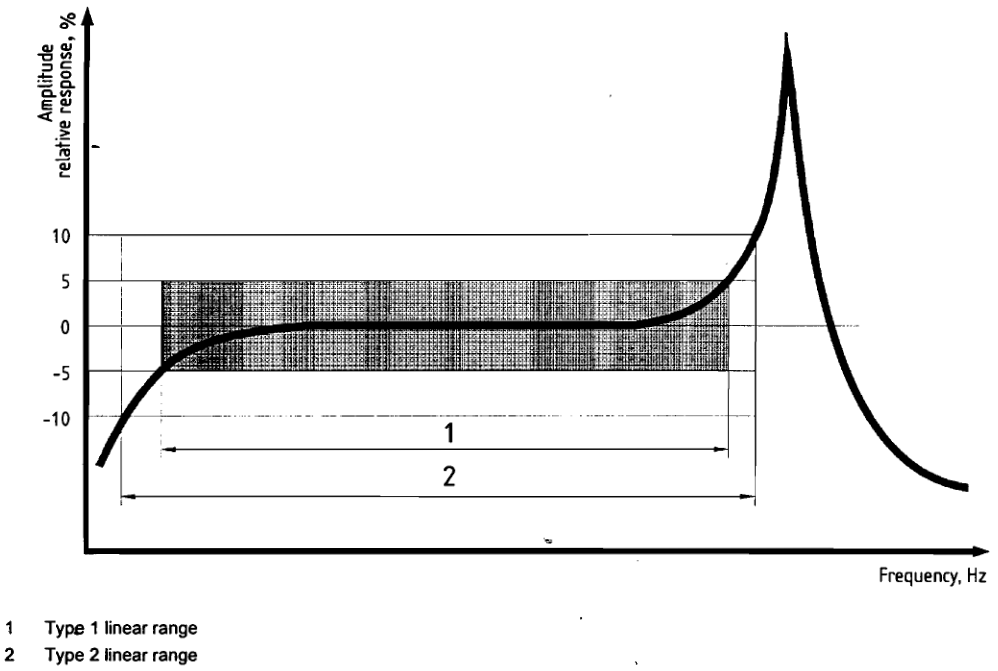
\includegraphics[width=0.8\textwidth]{assets/transducer-response.png}
	\caption{The transducer linear response and resonance in tolerance intervals~\cite{noauthor_iso_2002}}
	\label{fig:tranducer-response}
\end{figure}

Broadband measurement requires ``frequency ranges of 0.2 times the lowest rotational frequency to the highest frequency of interest''~\cite{noauthor_iso_2002}, not exceeding 10 kHz, with RMS velocity 0.1 - 100~mm/s. Bearings and gears diagnosis may push the upper-frequency limit even higher. The tolerances of amplitude and frequency calibrations fall into two types with allowable tolerances of $\pm 5 \%$ or $\pm 10 \%$~(Fig.~\ref{fig:tranducer-response}).

Equipment's ``health'' can be mischaracterized when there are significant differences in the machine's normal operating conditions. Baseline measurements in all acceptable conditions are to be acquired to reduce the error in vibration evaluation. According to the bathtub curve~(Fig.~\ref{fig:bathtub-curve}) reference signatures should be obtained after the initial part wear-in period. The reference spectral mask of the baseline condition is designed if maximal acceptance amplitudes are different for each significant frequency band ~\cite{ziaran_technicka_2013}.

The vibration baseline is defined by broad-band magnitudes and phases of motion vectors, the waveform in the time and frequency domain, the rotational speed of the machine as well as its frequency response to different speeds during start-up and coast-down captured in the Bode plot and waterfall plot. Changes during the machine operation are then depicted in value trends. Trends can be shown of overall amplitudes or limited to frequency bands.
\section{Signal preprocessing}
The vibration signals in a factory environment are inherently full of disturbances from adjacent equipment or irregular movement during object manipulation in the surrondings. In addition, accelerometers suffer from systematic measurement errors in the form of zero-g offset and bias that originates from a constant force of gravity. These unavoidable distortions are suppressible to some extent with digital filters. In the preprocessing stage we consider detrending, noise reduction with adaptive filters, and time synchronous averaging to supress interference among components.

\subsection{Detrending}
The oscillatory motion should be centered around the zero level for further manipulation. The constant offset is eliminated simply by subtracting the overall average from the signal. Moreover high pass DC blocker infinite impulse response (IIR) filter of 1st order can adjust to shifts of the mean value (Equation~\ref{equ:iir-dc-blocker}). The transition band depends upon the choice of corner frequency $f_{3dB}$ (Fig.~\ref{fig:dc-blocker}).

\begin{equation} \label{equ:iir-dc-blocker}
y_k = (1 - \frac{\omega}{2}) \cdot (x_k  -  x_{k - 1}) + (1 - \omega) \cdot y_{k - 1}; \quad \omega = 2\pi \cdot \frac{f_{3dB}}{f_s}
\end{equation}

A steeper 3~dB attenuation band can be achieved by increasing the order of the filter. Then the cutoff frequency should be such that filter coefficients are fractional numbers to counteract rounding errors~\cite{tittelbach-helmrich_digital_2021}.

\begin{figure}[h]
	\centering
	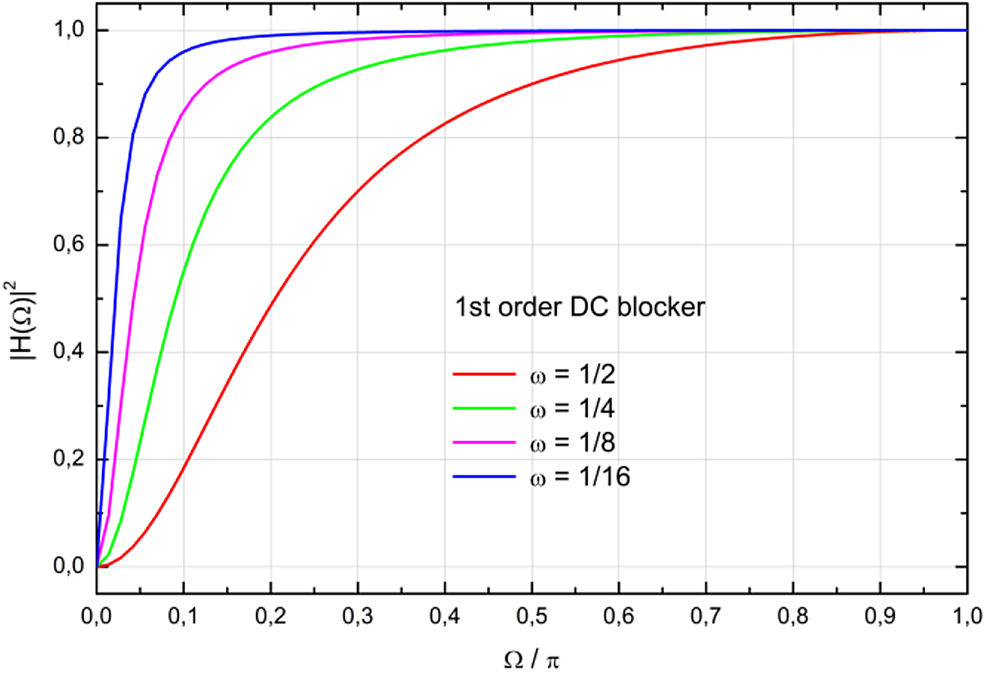
\includegraphics[width=0.7\textwidth]{assets/iir-1-dc-blocker-band.jpg}
	\caption{Transfer function of 1st order DC blocker filters ~\cite{tittelbach-helmrich_digital_2021}}
	\label{fig:dc-blocker}
\end{figure}

The finite impulse response (FIR) filter is not recommended for DC component removal because of the undesirable ripple effect with the small number of taps. Cascaded-integrator-comb (CIC) filters are proposed as an alternative instead~\cite{lyons_understanding_2011}.

\subsection{Adaptive noise cancellation}
Adaptive noise cancellation (ANC) involves an adaptive filter that self-adjusts coefficients through an update algorithm in response to the reference noise signal.  The objective of this filter is to minimize the cost function of mean square error (MSE) in error signal $e_k$ between signal contaminated with additive Gaussian noise $d_k$ and filter output $y_k$. Additive noise $n_k$ is assumed to be correlated with noise signal $\mathbf{X_k}$~\cite{diniz_adaptive_2020}.

Wiener-Hopf equations solve the optimal gradient of MSE function and FIR filter coefficient vector $\mathbf{W_k}$.  The least mean squares (LMS) algorithm recursively approximates this analytical solution with the method of steepest descent (Equation~\ref{equ:lms-adaptive-filter})~\cite{diniz_adaptive_2020}. The multiple parameters are to be considered in the evaluation of filter performance: convergence rate, estimated error, and signal-to-noise ratio (SNR).

\begin{ceqn}\begin{align} \label{equ:lms-adaptive-filter}
\mathbf{W}_{k+1} = \mathbf{W}_{k} + 2 \mu \mathbf{X}_{k}  e_k
\end{align}\end{ceqn}

The convergence stability is affected by step size $\mu$ which is bounded from above with the inverse of the maximal eigenvalue of input covariance matrix $\lambda_{max}$. The normalized least mean squares (NLMS) can handle input of varying scales  (Equation~\ref{equ:nlms-adaptive-filter}).

\begin{ceqn}\begin{align} \label{equ:nlms-adaptive-filter}
\mathbf{W}_{k+1} = \mathbf{W}_{k} + \frac{\mu}{\lVert\mathbf{X}_{k}\rVert^2} \mathbf{X}_{k}  e_k
\end{align}\end{ceqn}

\begin{figure}[h]
	\centering
	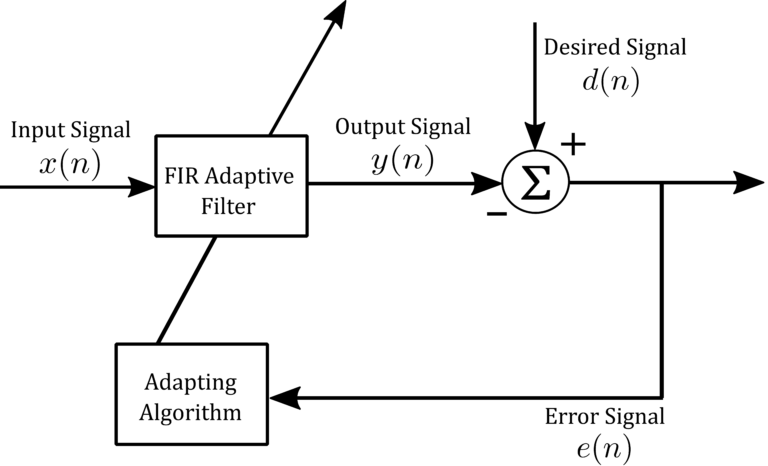
\includegraphics[width=0.8\textwidth]{assets/adaptive-filter.png}
	\caption{Adaptive noise cancellation filter diagram}
	\label{fig:adaptive-filter}
\end{figure}
\bigbreak

\subsection{Time synchronous averaging}
Time synchronous averaging is dimished the impact of sources unrelated to the harmonics of the rotational frequency in the vibrations. Time-domain waveform is averaged over $N$ points and aligned to synchronization pulse with period $T$ (Equation~ref{equ:tsa-average}). This technique has been successfully applied to the gearbox and bearing fault diagnosis~\cite{davies_handbook_2012,nandi_condition_2019}
\begin{ceqn}\begin{align}
x_{TSA} = \frac{1}{N} \sum_{n = 0}^{N - 1}{x(t + nT)}
\label{equ:tsa-average}
\end{align}\end{ceqn}

\section{Feature engineering}
Before the raw observations of the machine condition are input into a machine learning model, the descriptive and summarizing numerical attributes are calculated. The informative features are selected from the provided set to determine a diagnosis.

Among the main advantages of add-in extraction effort, as opposed to processing samples unmodified, is to gain better classification precision and reduce computational burden downstream through dimensionality reduction techniques. Predictive maintenance has ideal prerequisites for the application of feature engineering because the signal characteristics are pseudo-stationary, and the trend monitoring variables are established out of extensive domain expertise in mechanics.

The steps to undertake in the transformation of source data streams to a knowledge of machine status begins with
preprocessing that continues to feature extraction, then feature selection and the ultimate result is dependent on the model.

\subsection{Feature extraction}
% Feature Engineering for Machine Learning
\cite{zheng_feature_2018}
% Feature Engineering and Selection: A Practical Approach for Predictive Models
\cite{johnson_feature_2019}

% A Novel Online Machine Learning Approach for Real-Time Condition Monitoring of Rotating Machines
% - list of features
\cite{mostafavi_novel_2021}

% A New Statistical Features Based Approach for Bearing Fault Diagnosis Using Vibration Signals
% - knn with manhalobis distance
% - select features manually as oposed to CNN and RNN
\cite{altaf_new_2022}
$$X_{rms} = \sqrt{\frac{1}{N} \sum_{i=1}^{N}{x_i^2}}$$  % rms
$$X_{cf} = \frac{\max(|x_i|)}{X_{rms}}$$  % crest factor

$$ $$% standard deviation
$$X_{kv} = \frac{1}{N}  \sum_{i=1}^{N}{\frac{x_i - \bar{x}}{\sigma}} $$ % kurtosis


% Fault Detection of Bearing: An Unsupervised Machine Learning Approach Exploiting Feature Extraction and Dimensionality Reduction
% - Time domain: mean, standard deviation, rms (root mean square), peak value, peak-topeak value, shape indicator, skewness, kurtosis, crest factor, clearance indicator, etc. (ii) Frequency domain: mean frequency, central frequency, energy in frequency bands, etc. (iii) Time-frequency domain: entropy are usually extracted by Wavelet Transform, Wavelet Packet Transform, and empirical model decomposition.
\cite{brito_fault_2021}

FFT - Short Time Fourier Transform with Hamming window and Welch averaging
	% \cite{oulmane_automatic_2015}


% A large setof audio features for sound description
\cite{peeters_large_2004}
% Research on online intelligent monitoring system of band saw blade wear status based on multi‑feature fusion of acoustic emission signals
\cite{zhuo_research_2022}
% Early Detection of Imbalance in Load and Machine In Front Load Washing Machines by Monitoring Drum Movement
\cite{mohammadi_early_2020}
% A Data Mining based Approach for Electric Motor Anomaly Detection Applied on Vibration Data
\cite{egaji_data_2020}
% Condition Monitoring with Vibration Signals
\cite{nandi_condition_2019}

% Vibration Analysis for IoT Enabled Predictive Maintenance
\cite{jung_vibration_2017}

\paragraph{Statistical measures}
\begin{itemize}
\item Standard Deviation
\item Max. amplitude
\item RMS amplitude
\item Skewness
\item Kurtosis \\
---
\item Spectral centroid
\item RMS frequency
\item Root variance frequency
\item Spectral kurtosis / Fast kurtogram
\item Harmonics (peaks)
	% Multi-Scale Peak and Trough Detection Optimised for Periodic and Quasi-Periodic Neuroscience Data
	\cite{bishop_multi-scale_2018}
	% Non-Parametric Local Maxima and Minima Finder with Filtering Techniques for Bioprocess
	\cite{adikaram_non-parametric_2016}
	% Identification of harmonics and sidebands in a finite set of spectral components
	\cite{gerber_identification_2013}
	% Evaluation of Threshold-Based Algorithms for Detection of Spectral Peaks in Audio
	\cite{nunes_evaluation_2007}
\item Spectral Envelope
\item Harmonic spectral deviation \\
---
\item Energy
\item Spectral negentropy
	% Spectral negentropy and kurtogram performance comparison for bearing fault diagnosis
	\cite{avoci_spectral_2020}
\item TKEO - Teager-Kaiser energy operator
	%Application of Teager–Kaiser Energy Operator in the Early Fault Diagnosis of Rolling Bearings
	\cite{shi_application_2022}
\end{itemize}

\paragraph{Wavelet signal decompositions}

\begin{itemize}
\item CWT-SST - Synchrosqueezing Wavelet Transform
	% The fast continuous wavelet transformation (fCWT) for real-time, high-quality, noise-resistant time–frequency analysis
	\cite{arts_fast_2022}
	% A Concentrated Time–Frequency Analysis Tool for Bearing Fault Diagnosis
	\cite{yu_concentrated_2020}
	% Applications of the synchrosqueezing transform in seismic time-frequency analysis
	\cite{herrera_applications_2014}

\item WPD - Wavelet Packet Decomposition  - to approximation and detail coef. (Fejer-Korovkin wavelet)
	% Wavelet Packet Feature Extraction for Vibration Monitoring
	\cite{yen_wavelet_2000}
	% A wavelet approach to dimension reduction and classification of hyperspectral data
	\cite{wickmann_wavelet_2007}
	% The MFBD: a novel weak features extraction method for rotating machinery
	\cite{song_mfbd_2021}

\item EWT - Empirical Wavelet Transform - (Meyer wavelet)
	% Empirical Wavelet Transform - Gilles
	% On the computational complexity of the empirical mode decomposition algorithm
	\cite{wang_computational_2014}
	% Novel self-adaptive vibration signal analysis: Concealed component decomposition and its application in bearing fault diagnosis
	\cite{tiwari_novel_2021}
	% The MFBD: a novel weak features extraction method for rotating machinery
	\cite{song_mfbd_2021}
	% Fault Feature Extraction and Enhancement of Rolling Element Bearings Based on Maximum Correlated Kurtosis Deconvolution and Improved Empirical Wavelet Transform
	\cite{li_fault_2019}
	% An Improved Empirical Wavelet Transform for Noisy and Non-Stationary Signal Processing
	\cite{zhuang_improved_2020}
	% Time and frequency domain scanning fault diagnosis method based on spectral negentropy and its application
	\cite{yonggang_time_2020}
	% An Adaptive Spectrum Segmentation Method to Optimize Empirical Wavelet Transform for Rolling Bearings Fault Diagnosis
	\cite{xu_adaptive_2019}
	% Improved empirical wavelet transform (EWT) and its application in non‑stationary vibration signal of transformer
	\cite{ni_improved_2022}
\end{itemize}


\subsection{Feature transformation}
\cite{zheng_feature_2018}
\begin{itemize}
\item Normalization (min-max, standardize)
\item Log transformation (Box-Cox Transform) to normal distribution
\item Principal Component Analysis (PCA)  % \cite{brito_fault_2021}
\end{itemize}

\subsection{Feature selection}
Subset generation % p.193
Subset evaluation
Stopping criteria
Validation

\cite{nandi_condition_2019} % p.192
Filter method - SelectKBest  in evaluation phase
\begin{itemize}
\item Variance Threshold
\item Pearson correlation
\item ANOVA F-value
\item Mutal information
\item Fisher score
\item Spectral feature selection algorithm (SPEC)
\end{itemize}

\section{Diagnostics techniques} \label{section:diagnostics-techniques}
Fault identification in the rotating machinery is a one-class or multi-class classification problem acting in a semi-supervised manner because labels for degraded conditions are scarce in practice. The automation goals in monitoring can be broadly categorized as anomaly detection and recognizing the momentary fault type.

The guiding principles for algorithm selection are simplicity in terms of their straightforward visual explanation for the production managers, and the ability to progressively improve the model on the streaming data to address peculiarities in individual machine constructions.

\subsection{Novelty detection}
Anomaly, novelty, or outlier detection determines whether a health status deviates considerably from the baseline profile. The expert can then step in and diagnose the machine after the notice. Anomaly is a rare observation different from the others, raising suspicion that it was created by unrelated behavior~\cite{aggarwal_outlier_2016}. The observations get assigned anomaly scores, and those over the threshold are novelties.

The measurements coming in the steaming fashion have to be processed in a single pass. The detection model must deal with the minimal admissible assumptions about the nature of the input events. The outliers are derived based on non-parametric statistical models, nearest-neighbor clustering, and isolation-based approaches~\cite{gervasi_anomaly_2020}.
\bigbreak

\textbf{DenStream} is a density-based algorithm adapted from DBSCAN to cluster streaming data of arbitrarily shaped groups. Samples it includes in the first step into coherent clusters are core data points in each other's neighborhoods. Core points have at least \emph{MinPts} ($\mu$) points in their neighborhood of radius \emph{Eps} ($\varepsilon$) units. Then non-core points in the proximity area of the core point are attached to the cluster containing it~\cite{aggarwal_data_2014}.

Quality of clustering results is evaluated by \emph{Silhouette score} in the range [-1; 1]. It demands points within clusters to have high cohesion and at the same time to have large separation from other clusters. The low score indicates a too small or too large number of clusters~\cite{rousseeuw_rousseeuw_1987}. 

\begin{figure}[ht]
    \centering
    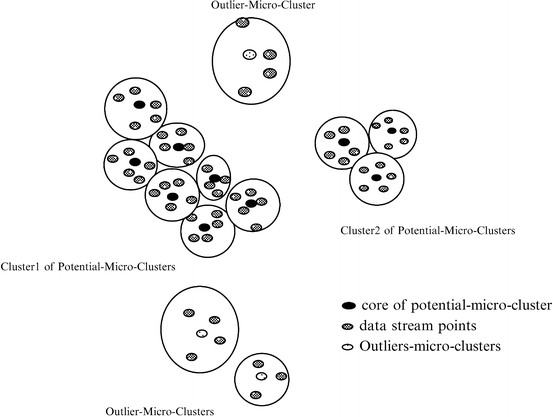
\includegraphics[width=0.8\textwidth]{assets/analysis/DenStream.png}
    \caption{DenStream~\cite{amini_density_2012}}
    \label{fig:denstream}
\end{figure}

In the online maintenance phase, DenStream summarizes the nearby observations into core \emph{micro-clusters} that can be potential micro-clusters or outlier \emph{micro-clusters} (Fig.~\ref{fig:denstream})~\cite{ghesmoune_state---art_2016}. The (outlier) \emph{o-micro-clusters} can grow into (potential) \emph{p-micro-clusters} when they encompass $\beta \mu$ points. The outliers are discounted after some time in accordance to the decay function: $f(t) = 2^{-\lambda t}$ or below the lower weight limit $\xi$. The on-demand offline stage runs DBSCAN over the approximate representation in micro-clusters to deliver final apportionment~\cite{cao_density-based_2006}.
\bigbreak

\textbf{Half-Space Tree} (HS-Tree) stands upon the concept of Isolation forest. It assumes that random splitting of each axis in the feature space will isolate outliers to their separate divisions sooner than non-deviant observations~\cite{gervasi_anomaly_2020,torres_automatic_2022}. This ensemble of trees is better suited for batch setting. HS-Tree stands out in adapting to changing streams because it is trained solely on normal data, requires constant memory, and is faster than density-based methods~\cite{tan_fast_2011}.

\begin{figure}[ht]
    \centering
    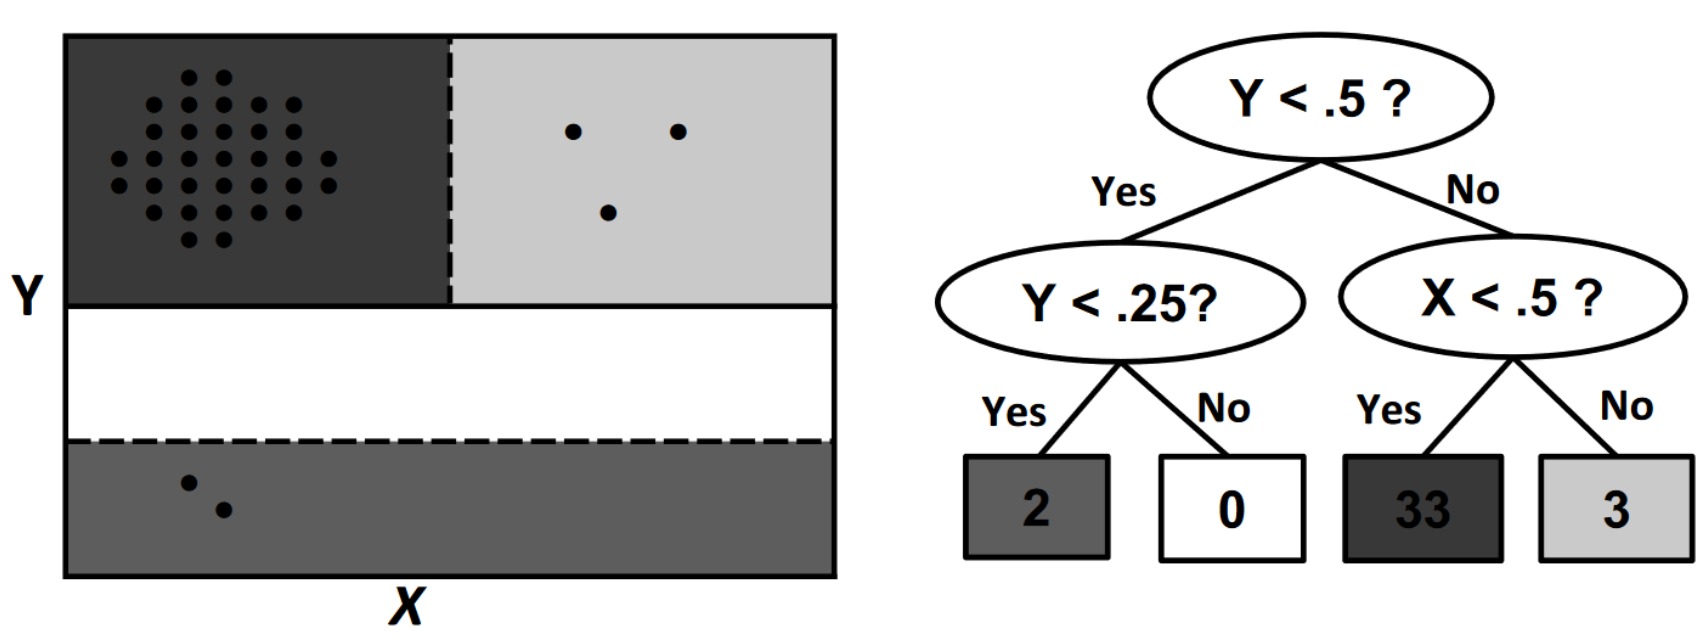
\includegraphics[width=0.8\textwidth]{assets/analysis/HS-Tree.png}
    \caption{Half-space tree~\cite{tan_fast_2011}}
\end{figure}

A full binary tree is built before the novelty detection begins by splitting tree nodes along the divisions in the randomly chosen perpendicular planes. The node stores its depth, value limits of the axis bisection (half-space), count of contained data points (mass) in two consecutive windows, and links to both child nodes~\cite{tan_fast_2011}. 

The anomaly profile in the latest window is always compared to the predecessor reference window. After the latest window is filled up, it replaces the reference window. It suffices to use a window size of 250 and an ensemble of 25 trees~\cite{tan_fast_2011}.

\subsection{Classification}
Accurate multi-class classification of machine fault causes according to the characteristics of known ones is a much more difficult task than novelty detection. Fault combinations have to be recorded and transformed into feature space. Interactions among fault root causes have to be considered. We are aware of rapid advances in knowledge transfer for deep neural networks~\cite{maurya_condition-based_2021}. So far, solutions seem not production-ready and hard to explain. Therefore, we opt to use a simpler model.

Performance of classification is estimated by several metrics on the validation set obtained using hold-out or cross-validation techniques. Frequently used quantities for classifier model evaluation include accuracy, precision, recall, f1 score, area under the ROC curve, and counts of hits and misses in a confusion matrix.
\bigbreak

\textbf{K-nearest neighbors} (kNN) assigns the data point to the class where the majority of $k$ closest instances belong (Fig.~\ref{fig:KNN}). It means it can work in a semi-supervised environment because it can infer labels just from knowing a few annotations. The major drawback of KNN is a preference for the majority class in imbalanced class-size datasets~\cite{shi_improving_2020}. The issue is mitigated with class weights or resampling classes by oversampling or undersampling. The KNN algorithm requires features to be normalized to assign the same importance to each predictor.

\begin{figure}[ht]
    \centering
    \begin{subfigure}[b]{0.49\textwidth}
        \includegraphics[width=\textwidth]{assets/analysis/KNN.png}
        \caption{KNN with k = 5}
        \label{fig:KNN}
    \end{subfigure}
    \hfill
    \begin{subfigure}[b]{0.49\textwidth}
        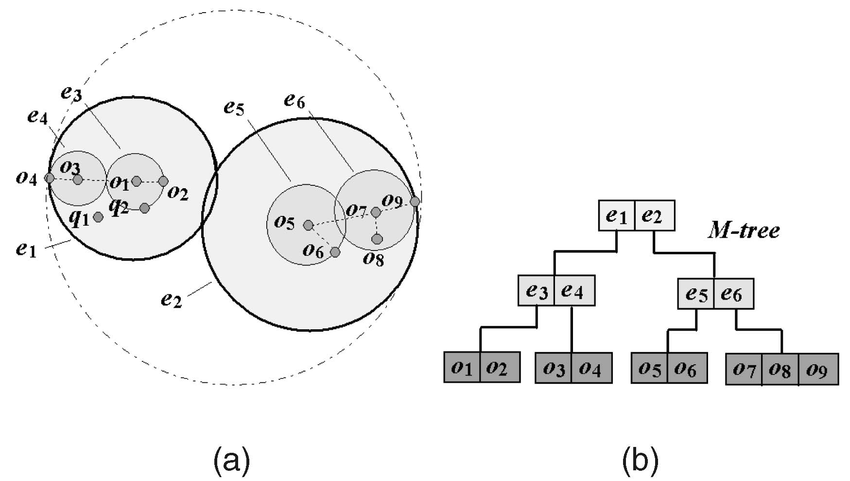
\includegraphics[width=\textwidth]{assets/analysis/M-tree.png}
        \caption{M-tree data structure}
        \label{fig:m-tree}
    \end{subfigure}
    \caption{Nearest neighbors classification algorithm~\cite{chen_skyline_2009}}
\end{figure}

The sense of distance between feature vectors $\mathbf{x}$, $\mathbf{y}$ have to be defined, so several metrics are available like \emph{Euclidian distance}, \emph{Mahalanobis distance}, \emph{Manhatann distance} etc. (Tab.~\ref{tab:KNN-distance})~\cite{sheng_review_2020, abu_alfeilat_effects_2019}. The optimal $k$ parameter is set by supervised learning according to the breaking point in the elbow curve that plots choices of $k$ against the error rate. The demanding neighborhood queries are sped up using spatial index in spatial databases that utilizes search tree such as kd-tree, R-tree, or M-tree.

\begin{table}[ht]
\centering
\renewcommand{\arraystretch}{2}
\begin{tabular}{|l|l|}
\hline
\textbf{Distance}     & \textbf{$d(\mathbf{x}, \mathbf{y})$}                                   \\ \hline
Manhatann distance	 & $ |x_i - y_i| $													   \\ \hline
Euclidian distance    & $ \sqrt{\sum_{i = 1}^{n}(x_i - y_i)^2} $                               \\ \hline
Mahalanobis distance  & $ (\mathbf{x} - \mathbf{y})^T C^{-1} (\mathbf{x} - \mathbf{y}) $       \\ \hline
\end{tabular}
\caption{Distance metrics for KNN}
\label{tab:KNN-distance}
\end{table}

The nearest-neighbor classifier has been successfully applied in machinery fault diagnostics. On the CWRU bearing dataset, the KNN with the accuracy of 96.2\% slightly outperformed SVM (95\%) on the combination of time and frequency-domain features, time-domain features - KNN 91.2\%, SVM 88.8\%, and frequency domain features - KNN (98.8\%), SVM (96.2\%)~\cite{jamil_feature-based_2021}. 

Comparison of KNN and KLDA on a feature set consisting of average, kurtosis, skewness, and standard deviation vectors in each domain has been conducted, achieving a data reduction rate of 95\%. Best accuracy was reached for PSD features with 99.13\% with KLDA and 96.64\% with KNN classifiers and Mahalanobis metric. The sampling frequency was set at 40 kHz~\cite{altaf_new_2022}. Despite KNN lagging in accuracy, we have to keep in mind annotations for faults were complete, and machine learning was not tested in a streaming context.

\subsection{Incremental learning}
Online or incremental machine learning operates on the streaming data, updating the model parameters with each new incoming event or in mini-batches. This approach finds its use in big data processing when the whole dataset is not available in advance or cannot be processed at once because of memory limitations. 

There are some additional obstacles to watch out for with incremental learning in comparison to batch learning~\cite{gepperth_incremental_2016}:

\begin{enumerate}
    \itemsep0pt

    \item \textbf{Concept drift} is defined as the change in data distribution function over time. The two types of concept drift are virtual and real. In virtual drift, changes occur only in the input distribution. Real drift means that the alteration comes to underlying functionality. Concept shift occurs with an abrupt change.

    \item \textbf{Stability-plasticity tradeoff} concerns the speed with which the model adapts to new information. The model can react quickly, making it less stable, or retain patterns for longer but become irresponsive to sudden shifts.

    \item \textbf{Model complexity} should be adjustable to ensure flexibility in unforeseen circumstances. Simpler models in the ensemble can also further increase prediction robustness. Resource limitation bound complexity from above.

    \item \textbf{Memory model} can store aggregates from seen observations and its typical examples or finite window of latest samples with forgetting factor.
\end{enumerate}


\textbf{Model benchmarking} in incremental learning is achieved by comparing models to their batch counterparts or using progressive validation~\cite{blum_beating_1999, halford_correct_2020}. It has been shown that incremental clustering algorithms have overall worse accuracy than batch versions~\cite{gepperth_incremental_2016}. In the validation process, precautions should be taken to prevent data leakage from future events into the past.

\begin{figure}[ht]
    \centering
    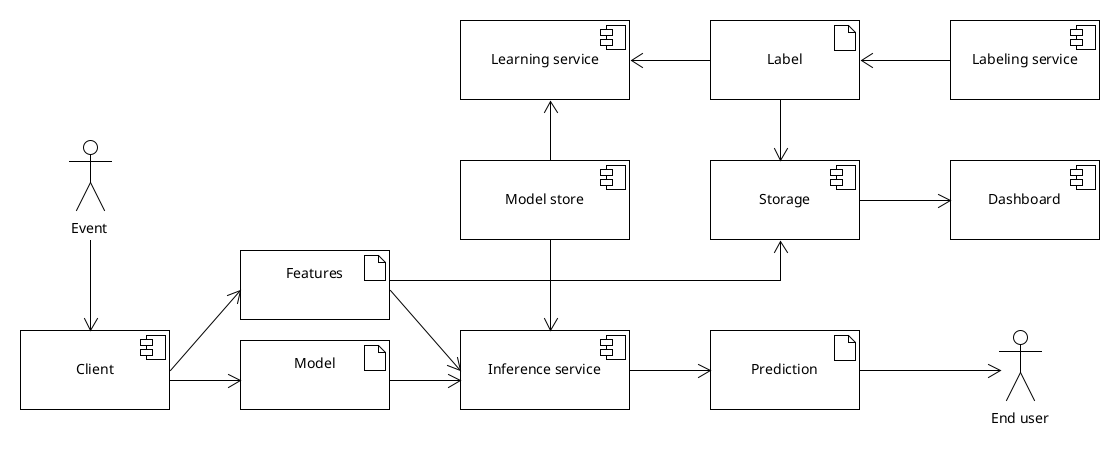
\includegraphics[width=\textwidth]{assets/analysis/incremental-learning.png}
    \caption{Incremental learning deployment architecture~\cite{gaia_online_2022}}
    \label{fig:online-learn-arch}
\end{figure} 

Deployment of an online machine learning model alongside supporting services is different from in established MLOps processes. Model store and Inference service components are supplemented with Labelling and Learning service~\cite{gaia_online_2022}. Their goal is to tune model parameters gradually as additional ground truth labels are provided. Labels can be provided later in a scheme called ``log and wait'', but data features are stored until such time.
  

\section{Evaluation datasets} \label{section:evaluation-datasets}
The experimentally designed features' relevancy is first proven in comparison to comprehensive benchmark datasets. There are a few standardized datasets used in the related work, e.g. \cite{ribeiro_rotating_2017}.

\emph{MaFaulDa} dataset combines vibration and acoustic measurements of the shaft in deviating positions and bearings abnormalities. \emph{CWRU dataset} focuses solely on faults in ball bearings. Another less known dataset concerns shaft unbalance, but compared to the previous two, it demonstrates behavior during revolution speed up.  

\subsection{Machinery Fault Database}
MaFaulDa\footnote{\url{https://www02.smt.ufrj.br/~offshore/mfs/page_01.html}} is a collection of 1951 multivariate time series for 4 different operational conditions on rotor kit Alignment Balance Vibration Trainer (ABVT)~(Fig.~\ref{fig:mafaulda-simulator}). Each series has 5~seconds in duration and is captured at 50 kHz. Vibration signals were obtained with piezoelectric accelerometers with a linear response up to 10~kHz, amplitude range to $\pm$490 $m/s^2$, and resolution step of 10.2~mV per $m/s^2$. 

\begin{figure}[h]
\centering
\begin{subfigure}[b]{0.48\textwidth}
	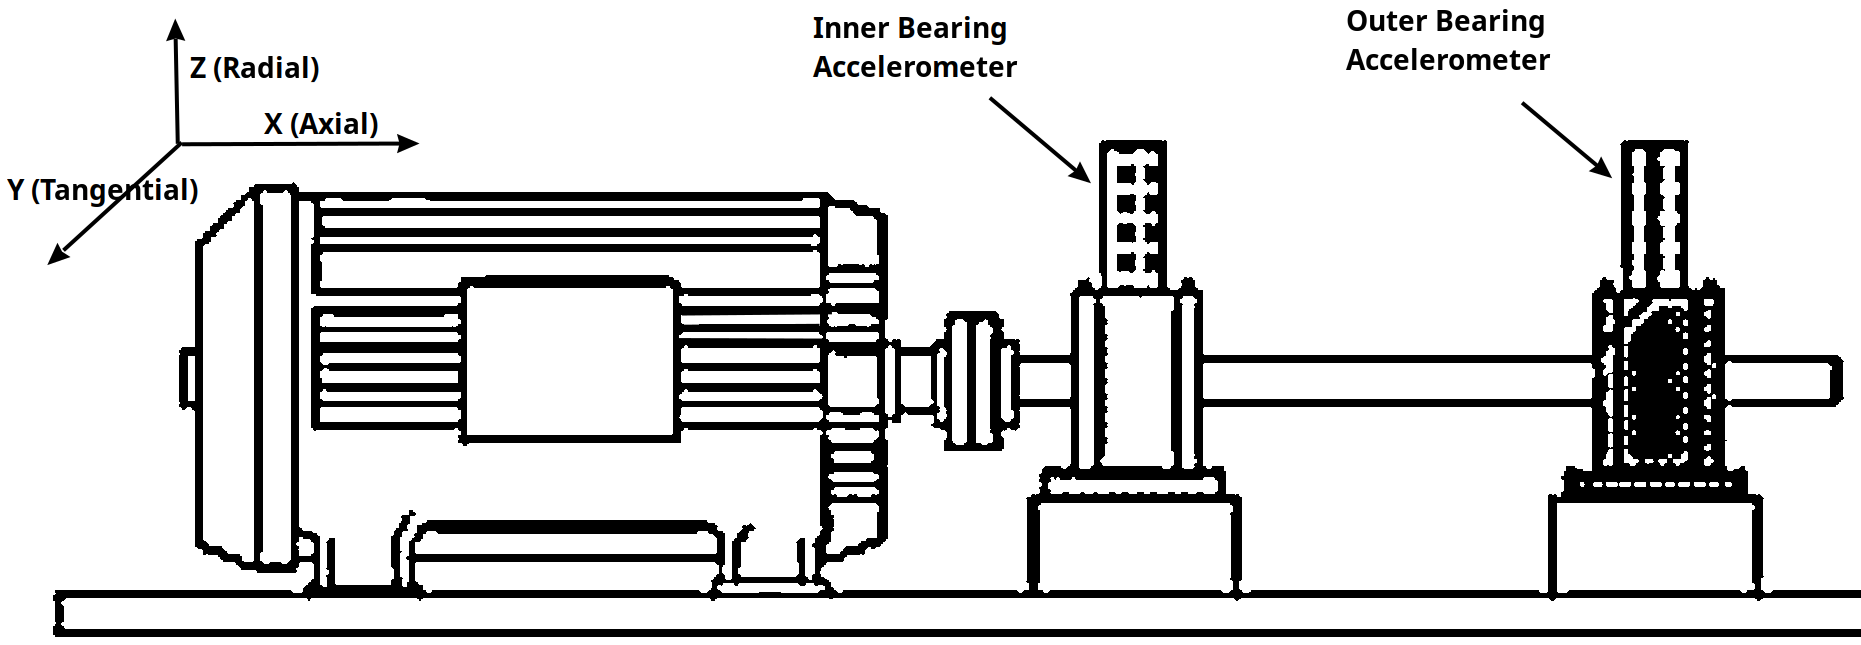
\includegraphics[width=\textwidth]{assets/mafaulda-simulator.png}
	\caption{Schematic diagram \cite{pestana-viana_influence_2016}}
\end{subfigure}
\hfill
\begin{subfigure}[b]{0.48\textwidth}
	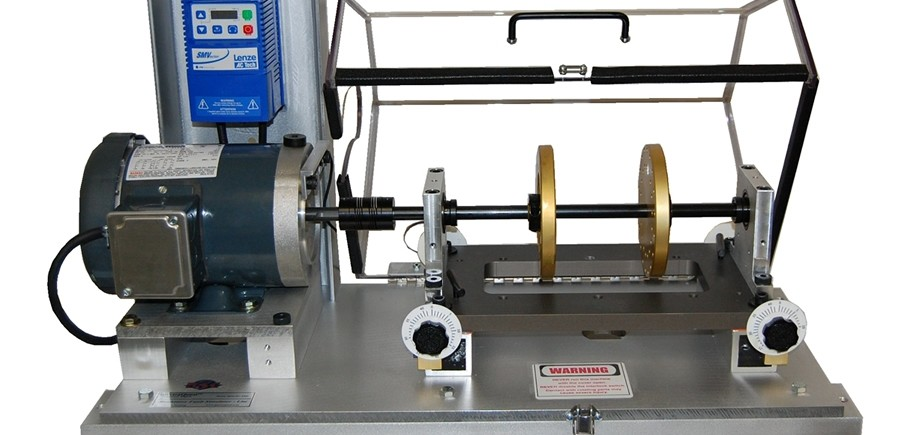
\includegraphics[width=\textwidth]{assets/machinery-fault-simulator.jpg}
	\caption{Mechanical construction \cite{noauthor_spectraquest_nodate}}
\end{subfigure}
\caption{Machinery fault simulator for MaFaulDa}
\label{fig:mafaulda-simulator}
\end{figure}

Observations were conducted in three cardinal axes simultaneously with 2 sets of accelerometers each one associated with one bearing (inner and outer bearings)~(Fig.~\ref{fig:mafaulda-simulator}). Additionally, a magnetic tachometer produced a pulse on shaft turn. The cardioid condenser microphone recorded sound emissions with a frequency range 20~Hz - 20~kHz. Sensors were fed into a four-channel dynamic signal acquisition module. 

Columns in the dataset are organized as depicted in table~\ref{tab:mafaulda-columns}. Machine rotational speeds were kept constant during a particular measurement, but covered a range from 737 to 3686~rpm with steps of approximately 60 rpm (equiv. 10~Hz - 60~Hz)~\cite{pestana-viana_influence_2016}. The maximal rotational frequency achieved with a high unbalance load is 3300 rpm.

\begin{table}[h]
\renewcommand{\arraystretch}{1.2}
\centering
\begin{tabular}{|l|l|}
\hline
\textbf{Columns} & \textbf{Description}                                                                                                                                               \\ \hline
1.               & \begin{tabular}[c]{@{}l@{}}Pulse with modulation of tachometer signal \\ to estimate rotation frequency  (in TTL levels)\end{tabular}                              \\ \hline
2., 3., 4.       & \begin{tabular}[c]{@{}l@{}}Underhang bearing accelerometer \\ (inner - between the rotor and motor)\\ - axial, radial, tangential direction\end{tabular}           \\ \hline
5., 6., 7.       & \begin{tabular}[c]{@{}l@{}}Overhang  bearing accelerometer \\ (Outer - outside most position after the rotor)\\ - axial, radial, tangential direction\end{tabular} \\ \hline
8.               & Microphone                                                                                                                                                         \\ \hline
\end{tabular}
\caption{MaFaulDa description of columns}
\label{tab:mafaulda-columns}
\end{table}

This database contains normal operating conditions, faults out of unbalance, horizontal and vertical shaft misalignment, and three types of faulty bearings in inner and outer positions: outer track, inner track, rolling elements~\cite{pestana-viana_influence_2016}.
\begin{itemize}
\itemsep0pt
\item \textbf{Normal} conditions are baseline without the adverse effect of fault in 49 different rotation speeds. 
\item \textbf{Unbalance} shaft time series uses 8 unbalancing weights from 6 to 35 grams and varying 45 - 49 speeds for each weight adding to 333 mass unbalance loads. 
\item \textbf{Vertical misalignment} set is comprised of 50 signals each (or 51 in one instance) obtained under displacements: 0.51, 0.63, 1.40, 1.90, 1.27, 1.78 mm.
\item \textbf{Horizontal misalignment} signals were recorded under displacements: 0.50, 1.00, 1.50, 2.00 mm, each with 49 different speeds (or 50 in one instance)~\cite{pestana-viana_influence_2016}.
\item \textbf{Bearing faults} are unnoticeable without unbalance. Therefore, weights of 6, 20, and 35 grams were attached to induce a detectable effect. Each unbalance mass was combined with cage, outer race, and ball faults at multiple rotation speeds, usually at 50 different speeds.
\end{itemize}


\subsection{CWRU bearings dataset}
In Case Western Reserve University (CWRU) bearing dataset\footnote{\url{https://engineering.case.edu/bearingdatacenter/download-data-file}} recordings were made of a fan end and drive end bearings under motor loads of 0, 1, 2, and 3~Horsepower (equivalently 0, 0.75, 1.49, 2.24~kW). Shaft speed was unaltered in all experiments, but it fluctuated between 1720 and 1797~rpm (approx. 29~Hz).

\begin{figure}[h]
\begin{subfigure}[b]{0.48\textwidth}
	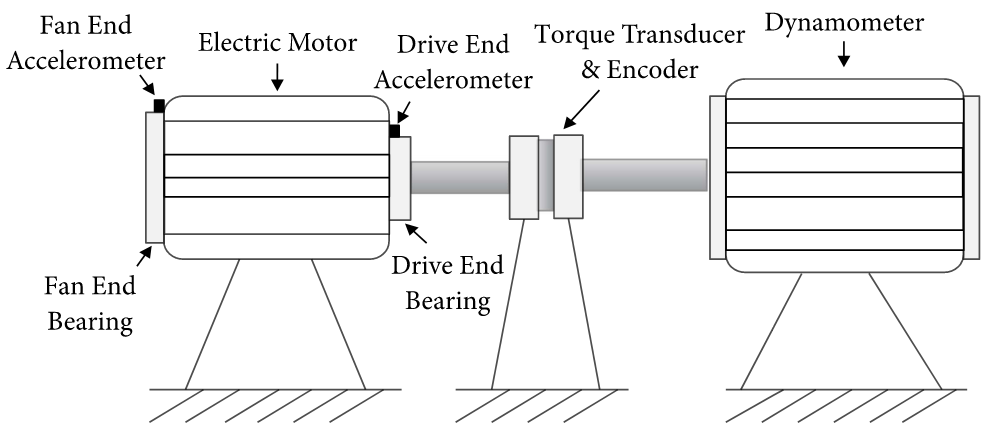
\includegraphics[width=\textwidth]{assets/cwru-test-stand-2.png}
	\caption{Schematic diagram \cite{song_bearing_2022}}
\end{subfigure}
\hfill
\begin{subfigure}[b]{0.48\textwidth}
	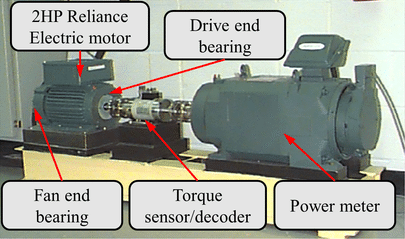
\includegraphics[width=\textwidth]{assets/cwru-test-stand.png}
	\caption{Mechanical construction \cite{yuhong_new_2021}}
\end{subfigure}
\caption{CWRU machine apparatus}
\label{fig:cwru-simulator}
\end{figure}

Single point defects were created with diameters of 0.007, 0.014, 0.021, 0.028, and 0.040 inches (equivalently 0.18, 0.36, 0.72, 1.02 mm). Fault locations on bearings are in the inner raceway, in the outer raceway directly and orthogonally relative to the load zone, and on rolling ball elements~(Fig.~\ref{fig:cwru-simulator})~\cite{jamil_feature-based_2021}. 

\begin{table}[h]
\centering
\renewcommand{\arraystretch}{1.2}
\begin{tabular}{|l|l|}
\hline
\textbf{Columns} & \textbf{Description}                 \\ \hline
1. DE        & Drive end accelerometer samples 		\\ \hline
2. FE        & Fan end accelerometer samples   			\\ \hline
3. BA        & Base accelerometer samples (optional)   \\ \hline
4. RPM     & Rotation speed of the motor in rpm        \\ \hline
\end{tabular}
\caption{CWRU dataset description of columns}
\label{tab:cwru-columns}
\end{table}

The sampling frequency during baseline set, drive end, and fan end bearing capture is 12 kHz, exclusively for drive end bearings samples were taken at 48 kHz. The duration of the time series is varied from 5 to 40 seconds. Drive end and fan end bearings signals are measured in each experiment. Accelerometer was sometimes mounted on the supporting base plate.

\subsection{Unbalance of the rotating shaft}
Unbalance Detection of a Rotating Shaft\footnote{\url{https://www.kaggle.com/datasets/jishnukoliyadan/vibration-analysis-on-rotating-shaft}} is a Kaggle dataset that simulates 4 different unbalance strengths. 
\begin{figure}[h]
\centering
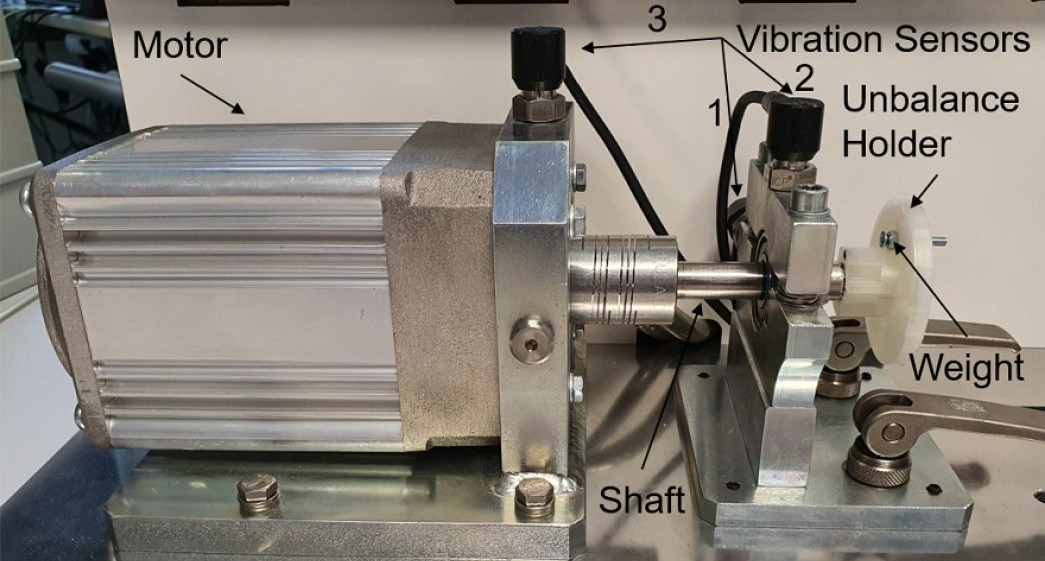
\includegraphics[width=0.7\textwidth]{assets/rotating-shaft.jpg}
\caption{Motor driving shaft in unbalance measurement \cite{mey_machine_2020}}
\label{fig:rotating-shaft}
\end{figure}

The setup is shown in Fig.~\ref{fig:rotating-shaft}. Mass of 3.28 grams (or 6.61 grams during severe unbalance test) is attached to unbalance holder successively in 5 sets (numbered 0 - 4) on the radii 0, 14, 18.5, 23, 23 mm. The rotation speed of the motor is perpetually rising between 630 and 2330 rpm in development datasets (marked with suffix D) and speeds from 1060 to 1900 rpm in the evaluation datasets (suffix E). The vibrations were recorded at a sampling rate of 4 kHz~\cite{mey_machine_2020}.

\begin{table}[h]
\centering
\renewcommand{\arraystretch}{1.2}
\begin{tabular}{|l|l|}
\hline
\textbf{Columns} & \textbf{Description}                      \\ \hline
1. V\_in         & Input voltage to the motor controller (V) \\ \hline
2. Measured\_RPM & Rotation speed of the motor (rpm)  \\ \hline
3. Vibration\_1  & 1. Vibration sensor (samples)             \\ \hline
4. Vibration\_2  & 2. Vibration sensor (samples)             \\ \hline
5. Vibration\_3  & 3. Vibration sensor (samples)             \\ \hline
\end{tabular}
\caption{`Unbalance on the rotating shaft' dataset description of columns}
\end{table}

The accelerometers used are piezoelectric and have a frequency range of up to 10 KHz, dynamic range of $\pm$490 $m/s^2$, and resolution step of 10.2~mV per $m/s^2$. These sensor parameters are the same as in the case of MaFaulDa. In total, three different uniaxial accelerometers are mounted on the motor housing.



\chapter{Design}

\section{Research questions}
\begin{enumerate}
\item \emph{Which time-frequency features can be extracted from vibrational signals to provide an accurate record of machinery faults?}
\item \emph{What are the savings in transmission bandwidth when chosen signal features are used in comparison to raw sampled measurement or lossless compression techniques?}
\item \emph{How can the machinery faults be continuously identified based on collected events?}
\end{enumerate}

\section{Infrastructure}
 \begin{itemize}
\item \textbf{Input:} Samples from acceleration in 3-axis, RPM, Noise background
\item \textbf{Output is either:} machine overall status, type of fault, remaining useful life
\item \textbf{Output for domain expert}: Annotation interface, Control chart of trend features, Power frequency spectrum, Waterfall plot
 \end{itemize}

\begin{enumerate}
\item MEMS accelerometers are placed on at least two distinict measurement points in two perpendicular axis and one sensor in base for denoising. Rotational speed is captured at the same time too.
\item Sensors are triggered in regular intervals (every 15 minutes) to collect sample recording from the band saw. Configurable parameters set based on experiments: sampling frequency, dynamic range, window type (Hamming) and size (based on resolution), PSD estimation method (Welch)
\item \textbf{Features} are computed and compared to recent measurements. If there is an statistically significant change the whole summary is send, otherwise keepalive notification is send.
\item Possible local communication between sensors to pre-compute clustering information
\item Database stores history of measurements
\item \textbf{Diagnosis panel runs clustering} with introduction of annotations to notify the operator about observed fault and imminent failure of the machine.
\end{enumerate}

Nároky na hardvér ako výstup analýzy - koprocesor (výpočet) - inštruckčná sada, real time odozva, ramka pri oknách



\chapter{Implementation} \label{chapter:implementation} 

\section{Data analysis}
% Jupyter notebook - TSFEL, numpy, pandas (data handling),  scipy (signal processing and stats),   | sklearn, imblearn | matplotlib


\section{Firmware}
% In C, ESP-IDF SDK and FreeRTOS tasks
% Found driver online
% Problems with timing - binary write (osciloscope pictures)
% tool for convert bin2csv


\begin{figure}[h]
    \centering
    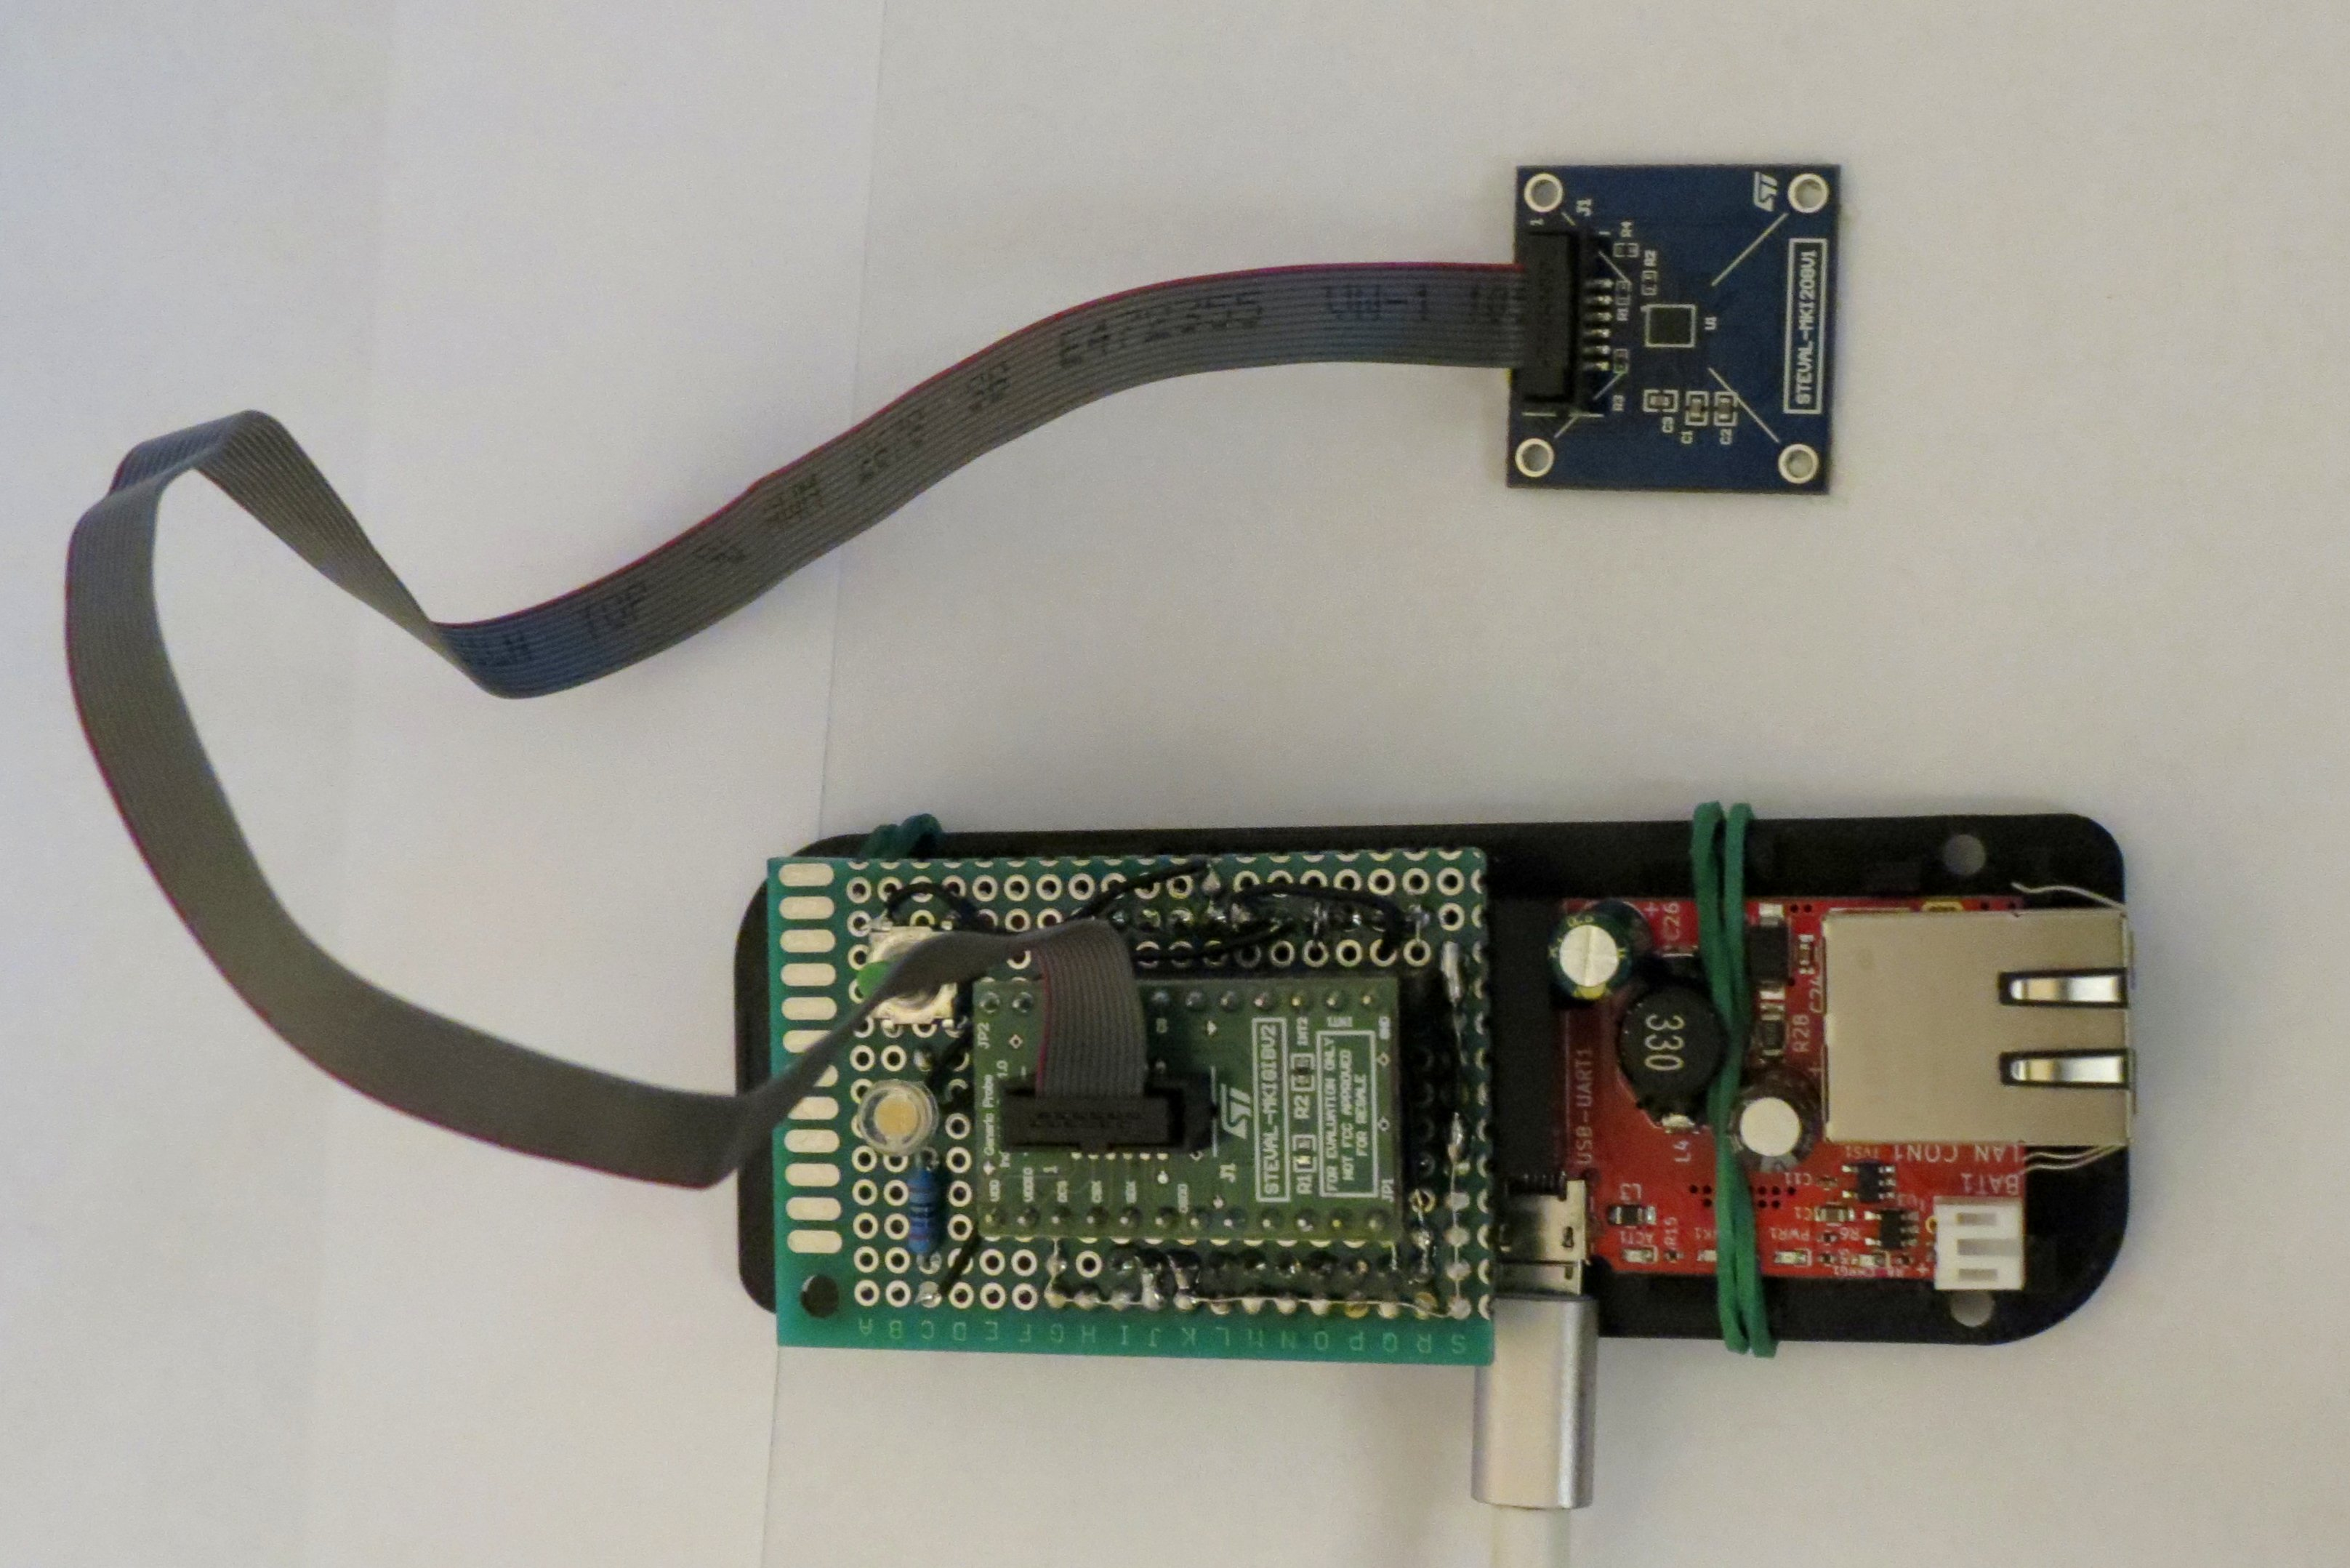
\includegraphics[width=0.5\textwidth]{assets/design/sensor/data-logger.jpg}
    \caption{Accelerometer Data Logger}
\end{figure}




\chapter{Conclusion} \label{section:conclusion}  
In the thesis we focused on trend indicator selection for an inexpensive industrial condition monitoring solution from vibration signals. The goal is to enable timely fault detection of machinery parts with as little input data as possible. For that purpose, we answer four research questions.

Attributes extracted to describe machine behavior come mainly from descriptive statistics, audio signal processing studies, and vibrodiagnostics technical standards (ISO 20186 and ISO 13343). These formulas compute 10 features summarizing the waveform in the temporal domain and 11 features characterizing spectral density estimation in 3 spatial directions \textbf{(RQ1)}.

In order to achieve more pronounced data savings, we choose the subset of 3 features in each domain by keeping the ones with the most similarity to the target variable. Feature selection metrics of the correlation coefficient, F statistic, mutual information, and their rank product are applicable in supervised learning. The features are squished from multiple dimensions using the Euclidian norm. Lossy compression ratios attained are 2381:1 for all features and 25000:1 for 6 features in the MaFaulDa dataset. We managed to discard more than 99.995\% of irrelevant data \textbf{(RQ2)}.

Feature subsets are subjected after normalization to a k-nearest neighbor classifier that ascertains their relative fault detection power. Because of model overtraining with small k, the feature triplets equal or slightly outperformed the whole set of features on the validation set with accuracy up to 10\%. The spectral features reach higher accuracies than temporal because of their smaller interdependency \textbf{(RQ3)}. 

The ensemble of feature selection with rank product produces the best model performance out of three combined in the majority of situations. No approach could find a triplet of predictors with an accuracy close to optimal one discovered exhaustively. Training on three principal components produced better accuracy than filtering feature selection, but PC mapping onto original trend indicators is unclear even in loading plots \textbf{(RQ3)}.

The considerable obstacle in an autonomous fault detection system deployment is the availability of labels for target variables. Annotations can be assigned belatedly or even never. Incremental learning kNN model on an unbalanced dataset on the whole feature set achieves at best 90\% accuracy with immediate feedback, 85\% with labels coming in 250 long tumbling windows, and 82\% with just 25\% of observations associated with the label. The comparable model trained in batch reaches an accuracy of 98\% \textbf{(RQ4)}.

Conclusions so far have been made on the MaFaulDa dataset imitating the realistic conditions. Therefore, in proper validation of the proposed solution in practice, we will compare it with the custom-made dataset. 

The vibration signals will be gathered on compressors in air conditioning units and water pumps in municipal pumping stations. We will develop firmware for sensor units capable of sampling accelerometers and saving measurements onto SD cards. The challenge awaits us in labeling samples themselves as it requires substantial expert knowledge. 

Feature selection methods should be incorporated into incremental learning. Hyperparameters shall be adjusted, and the balancing method used to increase model performance. The outlined tasks awaiting completion are planned for the DP~\rom{3} phase.

%\nocite{*}
\printbibliography[heading=bibintoc]

%  Appendix ---------------------------------------------------------
\addtocontents{toc}{\protect\setcounter{tocdepth}{0}}
\addtocontents{toc}{\cftpagenumbersoff{chapter}}
\let\svaddcontentsline\addcontentsline
\renewcommand\addcontentsline[3]{%
  \ifthenelse{\equal{#1}{lof}}{}%
  {\ifthenelse{\equal{#1}{lot}}{}{\svaddcontentsline{#1}{#2}{#3}}}}

\appendix
\titleformat{\chapter}{\normalfont\LARGE\bf}{Appendix \thechapter:}{0.5em}{}
\renewcommand{\chaptermark}[1]{\markboth{\MakeUppercase{Appendix \thechapter.\ #1}}{}}

% Resume
\thispagestyle{empty}
\chapter{Resume}
\pagenumbering{arabic}
\renewcommand*{\thepage}{A-\arabic{page}}


\clearpage


\thispagestyle{empty}
\chapter{Plan of work}
\pagenumbering{arabic}
\renewcommand*{\thepage}{B-\arabic{page}}

\section{Winter semester}

\begin{table}[h!]
\def\arraystretch{1.25}
\begin{tabular}{|l|p{12cm}|}
\hline
\textbf{Period} & \textbf{Work}                                                                                                                                                                                                                         \\ \hline
\nth{1} week         & Consultation with the supervisor on directions of the future work based on literature review during previous semester.
\\ \hline
\nth{2} week         & Outline the key sections of the analysis part in the thesis.
\\ \hline
\nth{3} week         & Match supporting literature with analysis sections. Further invesigation on the feature engineering methodology in condition monitoring.
 \\ \hline
\nth{4} week         & Summarize notes from condition monitoring articles and videorecordings of tutorials and conferences.
 \\ \hline
\nth{5} week         & Research transformation of vibration signal to feature space using time-frequency, harmonic and energy statistical metrics. Progress report meeting with the supervisor.
 \\ \hline
\nth{6} week         & Find articles and take notes about unsupervised and semi-supervised techniques in streaming data for machinery diagnostics, in order to gather information about suitable features.
 \\ \hline
\nth{7} week         & TBD (Narrow down wide variety applicable methods for signal decomposition)
 \\ \hline
 \nth{8} week         & TBD (Write thesis section on condition monitoring and machinery fault types)
 \\ \hline

\end{tabular}
\end{table}

\clearpage
\newpage


\section{Summer semester}

\clearpage


\thispagestyle{empty}
\chapter{Technical documentation} \label{appendix:technical-docs}
\pagenumbering{arabic}
\renewcommand*{\thepage}{C-\arabic{page}}

\section{Data collection plan}

The vibration measurements will occur monthly for pumps and biweekly for compressors from February 2024 until May 2024.
\begin{table}[ht]
\centering
\renewcommand{\arraystretch}{1.1}
\begin{tabular}{|l|l|p{0.6cm}|p{0.6cm}|p{0.6cm}|p{0.6cm}|p{0.6cm}|p{0.6cm}|}
\hline
\textbf{Machine}                                                                      & \textbf{Placement \textbackslash Month} & \multicolumn{2}{p{1.2cm}|}{\textbf{02/2024}} & \multicolumn{2}{p{1.2cm}|}{\textbf{03/2024}} & \multicolumn{2}{p{1.2cm}|}{\textbf{04/2024}} \\ \hline
\multirow{3}{*}{\textbf{\begin{tabular}[c]{@{}l@{}}Compressor\\ AC \#3\end{tabular}}} & SFTA001AT000TN                          &         &        &       &        &     &        \\ \cline{2-8} 
                                                                                      & SFTA002AT000TN                          &         &        &       &        &     &         \\ \cline{2-8} 
                                                                                      & Steel base (noise)                      &         &        &       &        &     &         \\ \hline
\multirow{3}{*}{\textbf{\begin{tabular}[c]{@{}l@{}}Compressor\\ AC \#5\end{tabular}}} & SFTA001AT000TN                          &         &        &       &        &     &         \\ \cline{2-8} 
                                                                                      & SFTA002AT000TN                          &         &        &       &        &     &         \\ \cline{2-8} 
                                                                                      & Steel base (noise)                      &         &        &       &        &     &         \\ \hline
\multirow{6}{*}{\textbf{\begin{tabular}[c]{@{}l@{}}Pump KSB\\ position \#1\end{tabular}}} & MTRA001AT090TN                          & \multicolumn{2}{p{1.2cm}|}{}                 & \multicolumn{2}{p{1.2cm}|}{}                 & \multicolumn{2}{p{1.2cm}|}{}                 \\ \cline{2-8} 
                                                                                      & MTRA002AT000TN                          & \multicolumn{2}{p{1.2cm}|}{}                 & \multicolumn{2}{p{1.2cm}|}{}                 & \multicolumn{2}{p{1.2cm}|}{}                 \\ \cline{2-8} 
                                                                                      & PMPA003AT000TN                          & \multicolumn{2}{p{1.2cm}|}{}                 & \multicolumn{2}{p{1.2cm}|}{}                 & \multicolumn{2}{p{1.2cm}|}{}                 \\ \cline{2-8} 
                                                                                      & PMPA004AT000TN                          & \multicolumn{2}{p{1.2cm}|}{}                 & \multicolumn{2}{p{1.2cm}|}{}                 & \multicolumn{2}{p{1.2cm}|}{}                 \\ \cline{2-8} 
                                                                                      & Motor base (noise)                      & \multicolumn{2}{p{1.2cm}|}{}                 & \multicolumn{2}{p{1.2cm}|}{}                 & \multicolumn{2}{p{1.2cm}|}{}                 \\ \cline{2-8} 
                                                                                      & Pump base (noise)                       & \multicolumn{2}{p{1.2cm}|}{}                 & \multicolumn{2}{p{1.2cm}|}{}                 & \multicolumn{2}{p{1.2cm}|}{}                 \\ \hline
\multirow{6}{*}{\textbf{\begin{tabular}[c]{@{}l@{}}Pump KSB\\ position \#7\end{tabular}}} & MTRA001AT090TN                          & \multicolumn{2}{p{1.2cm}|}{}                 & \multicolumn{2}{p{1.2cm}|}{}                 & \multicolumn{2}{p{1.2cm}|}{}                 \\ \cline{2-8} 
                                                                                      & MTRA002AT000TN                          & \multicolumn{2}{p{1.2cm}|}{}                 & \multicolumn{2}{p{1.2cm}|}{}                 & \multicolumn{2}{p{1.2cm}|}{}                 \\ \cline{2-8} 
                                                                                      & PMPA003AT000TN                          & \multicolumn{2}{p{1.2cm}|}{}                 & \multicolumn{2}{p{1.2cm}|}{}                 & \multicolumn{2}{p{1.2cm}|}{}                 \\ \cline{2-8} 
                                                                                      & PMPA004AT000TN                          & \multicolumn{2}{p{1.2cm}|}{}                 & \multicolumn{2}{p{1.2cm}|}{}                 & \multicolumn{2}{p{1.2cm}|}{}                 \\ \cline{2-8} 
                                                                                      & Motor base (noise)                      & \multicolumn{2}{p{1.2cm}|}{}                 & \multicolumn{2}{p{1.2cm}|}{}                 & \multicolumn{2}{p{1.2cm}|}{}                 \\ \cline{2-8} 
                                                                                      & Pump base (noise)                       & \multicolumn{2}{p{1.2cm}|}{}                 & \multicolumn{2}{p{1.2cm}|}{}                 & \multicolumn{2}{p{1.2cm}|}{}                 \\ \hline
\multirow{6}{*}{\textbf{Pump Sigma}}                                                  & MTRA001AT000TN                          & \multicolumn{2}{p{1.2cm}|}{}                 & \multicolumn{2}{p{1.2cm}|}{}                 & \multicolumn{2}{p{1.2cm}|}{}                 \\ \cline{2-8} 
                                                                                      & MTRA002AT000TN                          & \multicolumn{2}{p{1.2cm}|}{}                 & \multicolumn{2}{p{1.2cm}|}{}                 & \multicolumn{2}{p{1.2cm}|}{}                 \\ \cline{2-8} 
                                                                                      & PMPA003AT000TN                          & \multicolumn{2}{p{1.2cm}|}{}                 & \multicolumn{2}{p{1.2cm}|}{}                 & \multicolumn{2}{p{1.2cm}|}{}                 \\ \cline{2-8} 
                                                                                      & PMPA004AT000TN                          & \multicolumn{2}{p{1.2cm}|}{}                 & \multicolumn{2}{p{1.2cm}|}{}                 & \multicolumn{2}{p{1.2cm}|}{}                 \\ \cline{2-8} 
                                                                                      & Motor base (noise)                      & \multicolumn{2}{p{1.2cm}|}{}                 & \multicolumn{2}{p{1.2cm}|}{}                 & \multicolumn{2}{p{1.2cm}|}{}                 \\ \cline{2-8} 
                                                                                      & Pump base (noise)                       & \multicolumn{2}{p{1.2cm}|}{}                 & \multicolumn{2}{p{1.2cm}|}{}                 & \multicolumn{2}{p{1.2cm}|}{}                 \\ \hline
\end{tabular}
\end{table}
Each measurement will involve 3 trials for each position. The sensor is mounted to the machine with adhesive on double-sided carpet tape (placement notation follows MIMOSA convention from ISO~13373-1). After every trial, the sensor will be detached and attached again. 

The plan was consulted and approved by the machinery owners: VNET~a.s. and Bratislavská vodárenská spoločnosť,~a.s. Triaxial recording has a duration 60~s (at $f_s$ = 26.7 kHz) and a 16-bit resolution. The total space requirements for 108 recordings are 990 MiB.

% Ďalšie prílohy
% \input{chapters/appendix/B-technical-docs}
% Ak nechce vypísať čísla strán na konci prílohy: \cleardoublepage
	
%TODO: Digital medium
% \thispagestyle{empty}
\setcounter{figure}{0}
\chapter{Digital medium}
\pagenumbering{arabic}
\renewcommand*{\thepage}{C-\arabic{page}}
\par Evidenčné číslo práce v informačnom systéme: \RegNo
\par Obsah digitálnej časti práce (archív ZIP):
\par Názov odovzdaného archívu: 



\end{document}
